\documentclass{llncs}
\usepackage[utf8]{inputenc}				%% Für Umlaute in UTF-8-Kodierung
\usepackage{amssymb}					%% Für alle denkbaren mathematischen Symbole
\usepackage[german,english]{babel}		%% Für deutsche (und englische) Trennungsregeln und Bezeichnungen
\usepackage{hyperref}					%% Für Hyperlinks im PDF zum Anklicken
\usepackage{apacite}					%% Für Zitationsstil gem. APA
\usepackage{graphicx}
\usepackage{amsmath}
\usepackage[linesnumbered,ruled]{algorithm2e}
\usepackage[noend]{algpseudocode}
\usepackage{acronym}
\usepackage{tocbibind}
\setcounter{secnumdepth}{3}
\setcounter{tocdepth}{3}

\begin{document}
\tableofcontents
\begin{acronym}[Bash]
	\acro{KDE}{K Desktop Environment}
	\acro{SQL}{Structured Query Language}
	\acro{Bash}{Bourne-again shell}
	\acro{JDK}{Java Development Kit}
	\acro{VM}{Virtuelle Maschine}
	\acro{CGAN}Conditional Adversarial Networks
	\acro{PIX2PIX} Image-to-Image GAN
\end{acronym}
\selectlanguage{german}
\title{3-D Datenrekonstruktion mit generative Adverserial Networks}
\author{Andreas Wiegand}
\institute{Master These in künstlicher Intelligenz}
\maketitle								%% Titel setzen
%
\begin{abstract}		
Generative Adverserial Network(GAN) ist ein kün-stliches neuronales Netzwerk(ANN) aus dem Bereich der generativen Modelle. Die Aufgabe des GANs ist es, die Wahrscheinlichkeitsverteilung von Trainingsdaten zu erlernen und dadurch anschließend neue Samples aus dieser Wahrscheinlichkeitsverteilung zu generieren. Man erhofft sich, den hohen Datenaufwand beim trainieren von ANN zu umgehen und durch GANS neue Trainingsdaten zu generieren. Ziel dieser Arbeit ist es das Konzept von GANs auf 3D-Scans von Tabakblättern anzuwenden um die Wahrscheinlichkeitsverteilung von 3D-Daten zu erlernen. Ein weiteres Ziel ist es herraus zu finden ob mit Hilfe von GANs es möglich ist 3D-Daten welche beispielsweiße beim Scannen unvollständig sind ergänzen zu können. Im Folgenden wird auf die Theorie von GANs eingegangen, wie deren Aufbau und deren zugrunde liegendes mathematische Modell. Anschließend werden die Methoden des Experimentes präsentiert sowie die Ergebnisse diskutiert.  
\end{abstract}
%
\section{Einleitung}%

Um genaurer Prognossen über Erntemenge und frühzeitiger Erkennung von Krankheiten zu treffen werden 3D-Scan verfahren eingesetzt welche Pflanzen scannen und damit 3D-Daten liefern welche zur weiterverarbeitung von Machine-Learning Ansätzen benötigt werden. [EVLT BILD EINBAUEN UND GENAUER AUF SCANVERFAHRENE INGEHEN]. Jedoch sind diese Scanverfahren wie jede Informationsübertragung mit sogenannten rauschen verbunden das heißt die Information vom Empfänger zum Sender wird verändert und behält nicht die ursprünglichen Inhalt. Beispiele dafür waren ein Blatt verdeckt ein anderes Blatt und lässt die Sensoren des Scanner nicht zu das unter trunder liegende Blatt zu erfassen. Um nun nun diesen Verlust von Daten zu verhindert muss geprüft werden ob die Möglichkeit besteht diese Daten zu reparieren in dem sie ergänzt werden. In dieser Arbeit wird ein Ansatz überprüft welcher es Möglich machen kann dieses Verhalten zu erhalten.  Ein Ansatz der dafür Verwendet werden kann ist Deep Learning bei dem man das Deep Learning Modell den unterschied zwischen Reparierten und nicht reparierten Daten erlernt kann es rückschlüsse zeihen und selber Daten reparieren.
\\

Deep learning, however, gained much popularity across many academic disciplines
in recent years and has been used in computer vision successfully to
produce state-of-the-art results for various tasks. It is described as the application
of multiple processing layers to produce multiple levels of representation. It
is therefore capable of learning higher level representations of raw data, that can
be used for the intended task, e.g. classification of an image. The most common
realization are artificial neural networks (ANN) and especially convolutional
neural networks (CNN) for processing data with a grid-like topology, e.g. images.
Several publications have shown the effectiveness of CNNs for instance
segmentation of plant leaves on images (e.g. Ren and Zemel, 2016). But there
is a lack of research in applying deep neural networks to 3D representations of
plants.
\\

In den letzten Jahren haben sich im Deep Learning Bereich besonders die discriminativen Modelle hervorgehoben, welche Input Daten wie Bilder, Audio oder Text Daten zu bestimmte Klassen zuordnen. Der Grund für das steigende Interesse liegt in der niedrigen Fehlerrate bei discriminativen Aufgaben, im Vergleich zu anderen Maschine Learning Ansätzen, wie Desicion Trees oder Markov Chains\cite{Grundlagen}. Die Modelle lernen eine Funktion welche Input Daten X auf ein Klassen Label Y abbildet. Die Modelle werden dabei von ANN repräsentiert. Man kann auch sagen das Model lernt die bedingte Wahrscheinlichkeitsverteilung $P(Y|X)$ \cite{discrim}. Generative Modelle haben die Aufgabe die Wahrscheinlichkeitsverteilung von Trainingsdatendaten zu erlernen. Es lernt eine multivariate Verteilung $P(X,Y)$, was dank der Bayes Regel auch zu $P(Y|X)$ umgeformt werden kann und somit kann das Modell auch für discriminativen Aufgaben herangezogen werden. Gleichzeitig können aber neue (x,y) Paare erzeugt werden, was zu dem Ergebnis von neuen Datensätzen führt welche nicht Teil der Trainingssample sind \cite{discrim}. In diesem Paper wird speziel auf GAN, aus der Vielzahl von generativen Modellen eingegangen. Diese wurden von Goodfellow\cite{goodfellow2014} entwickelt und ebneten den Weg für Variationen, welche auf der Grundidee von GANs aufbauen. 2017 wurden alleine 227 neue Paper zu diesem Thema vorgestellt. Ein Grund weshalb GAN an Popularität gewinnt ist der, dass neuronale Netzwerke mit Zunahme der Trainingsdatenanzahl eine Erhöhung der Performance für die sie Trainiert werden zeigen. Was bedeutet,dass sich mit Zunahme der Datenanzahl die Chance auf eine bessere Performance der Neuronalen Netzwerke ergibt \cite{data}. An diesem Punkt erhofft man sich durch GANS mehr qualitative Daten zu erzeugen und somit das Trainingsergebnis zu discriminativen Modelle zu verbessern. 

\subsection{Objectives}

In den letzten Jahren haben sich im Deep Learning Bereich besonders die discriminativen Modelle hervorgehoben, welche Input Daten wie Bilder, Audio oder Text Daten zu bestimmte Klassen zuordnen. Der Grund für das steigende Interesse liegt in der niedrigen Fehlerrate bei discriminativen Aufgaben, im Vergleich zu anderen Maschine Learning Ansätzen, wie Desicion Trees oder Markov Chains\cite{Grundlagen}. Die Modelle lernen eine Funktion welche Input Daten X auf ein Klassen Label Y abbildet. Die Modelle werden dabei von ANN repräsentiert. Man kann auch sagen das Model lernt die bedingte Wahrscheinlichkeitsverteilung $P(Y|X)$ \cite{discrim}. Generative Modelle haben die Aufgabe die Wahrscheinlichkeitsverteilung von Trainingsdatendaten zu erlernen. Es lernt eine multivariate Verteilung $P(X,Y)$, was dank der Bayes Regel auch zu $P(Y|X)$ umgeformt werden kann und somit kann das Modell auch für discriminativen Aufgaben herangezogen werden. Gleichzeitig können aber neue (x,y) Paare erzeugt werden, was zu dem Ergebnis von neuen Datensätzen führt welche nicht Teil der Trainingssample sind \cite{discrim}. In diesem Paper wird speziel auf GAN, aus der Vielzahl von generativen Modellen eingegangen. Diese wurden von Goodfellow\cite{goodfellow2014} entwickelt und ebneten den Weg für Variationen, welche auf der Grundidee von GANs aufbauen. 2017 wurden alleine 227 neue Paper zu diesem Thema vorgestellt. Ein Grund weshalb GAN an Popularität gewinnt ist der, dass neuronale Netzwerke mit Zunahme der Trainingsdatenanzahl eine Erhöhung der Performance für die sie Trainiert werden zeigen. Was bedeutet,dass sich mit Zunahme der Datenanzahl die Chance auf eine bessere Performance der Neuronalen Netzwerke ergibt \cite{data}. An diesem Punkt erhofft man sich durch GANS mehr qualitative Daten zu erzeugen und somit das Trainingsergebnis zu discriminativen Modelle zu verbessern. 

\subsection{Outline}

Diese Arbeit ist folgender Maßen strukturiert. In Kapitel 2 "Grundlagen und ähnliche Arbeiten" werden theoretische Grundlagen welche für diese Arbeit benötigt wird genauer beleuchtet. Außerdem sollen vorrangegeganngen Arbeiten welche einfluß auf diese Ausüben vorgestellt werden um zu veranschaulichen aus welchen Gründen diese Funktioneren kann.
\\\\
Kapitel 3 - stellt die Arbeit an sich vor. Welche Methoden gewählt wurden ob diese zu Entwickeln und Auszuführen. Die Trainingsdaten werden vorgestellt und Modelle aufgezeigt.
\\\\
Kapitel 4 - Gibts  ausführliche Angaben über die Ergebnisse von den Experimenten und evaluiert sie für ihre Aussagekraft.
\\\\
Kapitel 5 - Gibt eine Zusammenfassung über die Arbeit und wird sie kritisch Diskutieren. Desweiteren wird ein Ausblick erstellt inwiefern das Ergebnis für zukünftige Arbeiten von relevanz ist. 

\section{Grundlagen und ähnliche Arbeiten}

Im folgenden Kapitel werden auf theoretische Grundlagen eingegangen, welche zum Verständnis dieser Arbeit benötigt wird. Zunächst werden generative Modelle im Allgemeinen vorgestellt, welche den Grundgedanken der Datengeneration für GANs aufzeigen und mit deren Hilfe es möglich gemacht werden soll unkenntliche beziehungsweise beschädigte Modelle von Objekten wieder herzustellen. Diese Theorie baut zunächst auf die Datenstruktur von künstlichen Neuronalen Netzwerken auf, welche durch verschiedene Modelle dargestellt werden können. Im Kapitel Conditional-GAN und 3D-GAN werden die theoretischen Grundbausteine der vorherigen Themen vertieft und bilden den Grundstein für das in dieser Arbeit vorgestellte verfahren zur 3D-Datenrekonstruktion von 3D-Modellen aus Tabakblättern. 

\subsection{Künstliche Neuronale Netzwerke}

Künstliche Neuronale Netzwerke(KNN) ist eine Datenstruktur welche von biologischen neuronalen Netzen wie sie bei Lebewesen vorkommen inspiriert sind. KNN haben das Ziel ein Funktion f* zu approximieren. Dabei werden Parameter $\Theta$ eines Models so angepasst, um die Abbildung von y = f(x;$\Theta)$ zu approximieren. Die Modelle werden auch als feedforward Neuronale Netzwerke betitelt weil der Informationsfluss des Models von Input zu Output fließt und keine Rekursion von Output zu Input statt findet. Diese Approximation wird durch Machine Learning Ansätzen erlernt man spricht auch von einen Optimierungsproblem. KNN können aus mehreren Schichten sogenannten Hidden Layer n besteht welche als f\textsuperscript{(n)} dargestellt werden und n >=1 sein muss. Ein 2-Layer KNN ist dann definiert durch f(x)=f\textsuperscript{(2)}(f\textsuperscript{(1)}(x)). Es gibt einen Input Layer welche den Input in das Netzwerk aufnimmt. Ein ANN mit mehr als nur 1 Layer und wird dies dies mit Maschine Learning trainiert spricht man auch von Deep Learning. Im vorherigen Beispiel ist dies f\textsuperscript{(1)} und der letzte Layer des Netzwerkes wird Output Layer genannt. Im vorherigen Beispiel ist das f\textsuperscript{(2)}\cite{Grundlagen}. In \ref{fig:Bild1} sind ein ANN exemplarisch dargestellt. Es soll die Konnektivität der einzelnen Layer veranschaulichen und den Informationsfluss von Input zu Output. 

\begin{figure}[htbp]
	\centering
	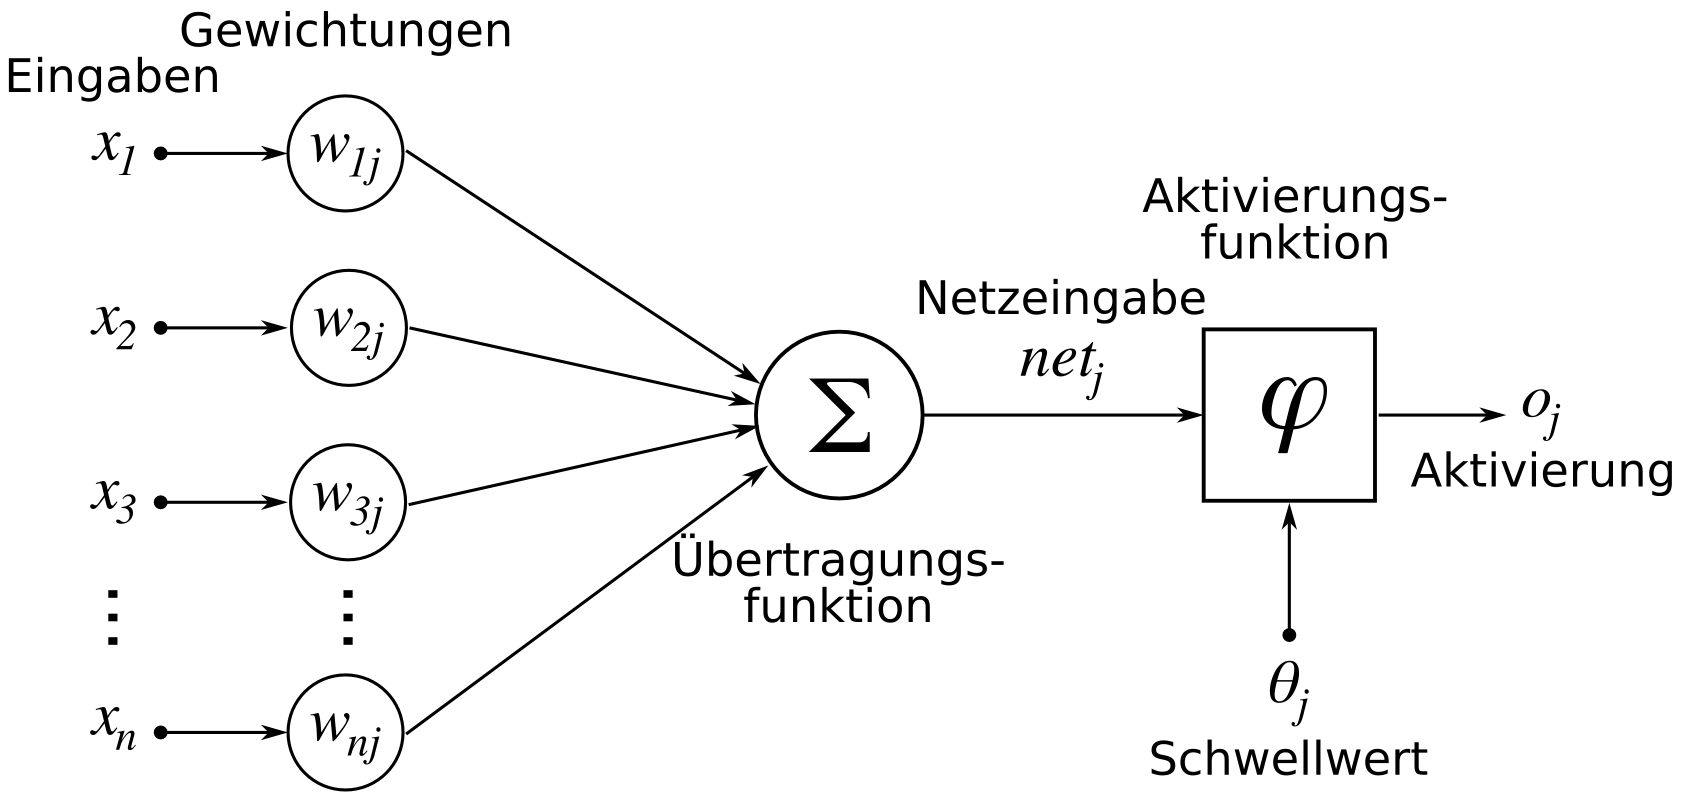
\includegraphics[width=1.0\textwidth]{Neuron.png}
	\caption{künstliches Neuron}7
	\label{fig:Bild1}
\end{figure}

Jeder Layer besteht aus künstliche Neuronen diese haben ihren Namensgebung von aus der Natur stammende Neuron in Gehirnen von Lebewesen. Neuronen sind die Bausteine aus denen die Gehirne von Lebewesen, wie Fische, Vögel, Säugetiere zusammen gesetzt sind. Neuronen oder auch Nervenzellen bestehen in eine Zellkern der Zentrum der Zelle um sie herum sind Dendriten. Neuronen sind untereinander mit den Axon verbunden, diese haben an den enden Synapsen welche die grenze von Axon zur Nervenzelle einen Spalt bilden. Dieser Spalt kann überwunden werden indem von der Synapse Botenstoffe abgesendet werden welche sich dann an Rezeptor der gegenüberliegenden Synapse anhaften. Diese Übertragung findet statt wenn an der Synapse ein bestimmter Schwellenwert überschritten hat wurde von elektrischen reizen welche die Zelle abfeuert lässt. Künstliche Neuronen haben diese Schwellenwert durch sogenannte Gewichte w\textsubscript{ij} diese sind auf den Verbindungen zwischen den Neuronen in den unterschiedlichen Layern im Netzwerk.
\begin{figure}[htbp] 
	\centering
	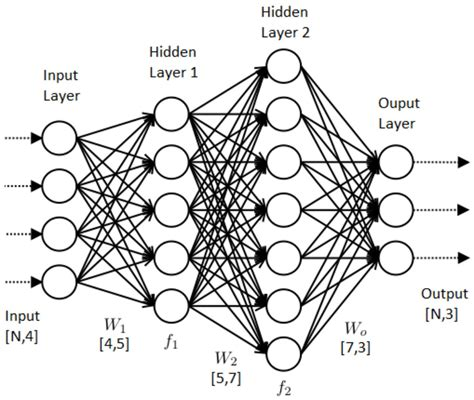
\includegraphics[width=1.0\textwidth]{neuronalesnetzwerk.jpg}
	\caption{künstliches neuronales Netzwerk}
	\label{fig:Bild2}
\end{figure}
\\
Jeder Layer eines KNN besteht aus mehreren Neuronen. Ein Neuron $\theta$ kann mehrere Input X\textsubscript{n} erhalten und produziert einen Output $\omega$\. Die Berechnungen welche von den Neuron durchgeführt wird ist zunächst jeden Input X\textsubscript{n} mit einen Gewicht w\textsubscript{ij} zu multiplizieren wobei. Anschließend wird die Summe von x*w gebildet. Das Ergebnis wird dann in eine Aktivierungsfunktion gegeben. Ein Neuron ist definiert durch:
\\\\
\begin{math}
y\textsubscript{k} = Aktivierungsfunktion(\sum_{j=0}^{m}(w\textsubscript{kj}+x\textsubscript{j})+b\textsubscript{k})                
\end{math}
\\\\
Die Aufgabe der Aktivierungsfunktion ist es eine nicht liniere Transformation des Inputs zu erzeugen. Damit kann das KNN nicht lineare Funktionen abbilden und somit komplexere Aufgaben lösen. Es gibt unterschiedliche Aktivierungsfunktionen Beispiele sind Sigmoid-Funktion
\begin{math}
\sigma(x)=\frac{1}{1+exp(-x)}
\end{math}
oder Softmax-Funktion 
\begin{math}
\zeta(x)\textsubscript{j} = \frac{e\textsuperscript{x\textsubscript{j}}}{\sum_{k=1}^{K}e\textsuperscript{x\textsubscript{k}}}
\end{math}
oder Rectified Linear Unit (ReLU)
\begin{math}
f(x)=\max(0,x) 
\end{math}
oder Leacky Rectified Linear Unit(Leaky Relu)
\begin{math}
f(x) = \begin{cases}
x  	 & \quad \text{if } x > 0\\
0.01x & \quad \text{sonst} 
\end{cases}
\end{math}
Der Funktionsplot von Softmax und Sigmoid kann in  Abb. \ref{fig:Bild3} und \ref{fig:Bild4} entnommen werden.
\begin{figure}[htbp] 
	\centering
	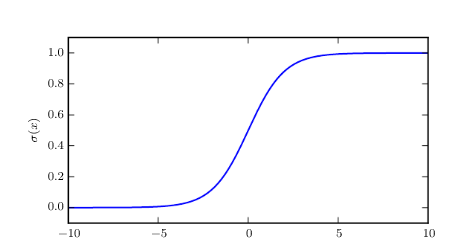
\includegraphics[width=1.0\textwidth]{sigmoid.png}
	\caption{Sigmoid Funktion}
	\label{fig:Bild3}
\end{figure}
\begin{figure}[htbp] 
	\centering
	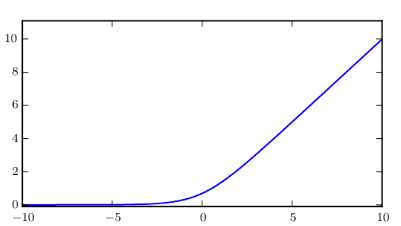
\includegraphics[width=1.0\textwidth]{softmax.png}
	\caption{Softmax}
	\label{fig:Bild4}
\end{figure}

\subsubsection{Backpropagation Algorithmus}\label{sec:test}

Um nun KNNs zu trainieren und den gewünschten Output y zu generieren wird der Backpropagation Algorithmus benutzt werden dieser zählt zu den Optimierungs- Algorithmen für KNN. Er konnte zeigen das dieser Algorithmus schneller und effizienter auf Neuronalen Netzwerken arbeitet als andere Optimierungsalgorithmen vor ihm. Das mathematische Zugrundeliegende Konzept ist ein Optimierungsproblem der die Partitiellen Ableitung von  $\frac{\partial Z}{\partial w}$, wobei Z die Zielfunktion und w die Gewichte im zu optimierenden Neuronalen Netzwerk sind. Für eine Funktion $f$(x) = y ist die Ableitung definiert als $f^\prime$(x) oder $\frac{dy}{dx}$ und gibt die Steigung der Funktion an Punkt x an. Durch die Steigung an Punkt x ist man nun in der Lage einer Änderung von der Ableitung x dahin gehen optimieren \cite{Grundlagen}. Dieses Verfahren kann dabei helfen Funktionen das KNN  dahingehen zu optimieren den gewünschten Output y zu erlangen. \\

Wenn nun $f^\prime$(x) = 0 haben wir keinerlei Information über die Steigung erreicht. Dies ist aber kein Indiz dafür sein das $f$ ein Optimum erreicht hat. Es könnten wie in Abbildung \ref{fig:Bild5} unten dargestellt ein lokales Minimum sein dass heißt das wir nur an diesen Punkt ein Minimum erreicht haben aber im Funktionsverlauf ein noch niedrigeres Minimum vorhanden ist. Oder einen Sattelpunkt welche ein Übergang zu einen anstieg der Funktion bildet.
Ist nun die die Funktion $f$ definiert als $f$: $\mathbb{R}$\textsuperscript{n} $\rightarrow$  $\mathbb{R}$ und hat als Input mehrere Variablen. Die partielle Ableitung $\frac{\partial f(x)}{\partial x\textsubscript{i}}$ zeigt an wie sehr sich $f(x)$ ändert wenn wir x\textsubscript{i} ändern. Der Gradient $\nabla\textsubscript{x}f(x)$ ist ein Vektor welche alle partiellen Ableitungen von $f$ enthält. Nun kann man f optimieren in dem man in die Richtung des Gradienten geht welche negativ ist. Dieses Verfahren wird Gradient Descent genannt \cite{Grundlagen}.
\begin{figure}[htbp] 
	\centering
	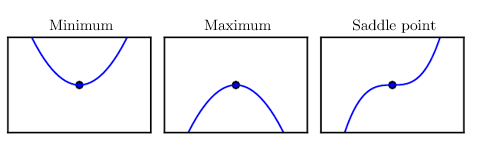
\includegraphics[width=1.0\textwidth]{saddle.png}
	\caption{Minimum Maximum Saddle Point}
	\label{fig:Bild5}
\end{figure}

Algorithmen die für Deep Learning eingesetzt werden, beinhalten eine Art von Optimierung, ohne diese ist eine Umsetzung des Lernprozesses nahezu unmöglich. Diese Minimierungs-funktionen oder auch cost function (welche in vielen Publikationen unterschiedlich bezeich-net wird „loss“- oder „error function“) wollen immer dasselbe Ziel: eine gewisse Target Funktion ermitteln, welche für einen Input den gewünschten Output ausgibt. Das Ziel ist in anderen Worten eine Menge an Gewichten und Biases zu finden, für welche, die quadrati-schen Kosten (C(w,b)) so gering wie möglich sind. Um dies zu erreichen, wird der Gradient Decient Algorithmus eingesetzt (Nielsen, 2017).
Der Grund des Einsatzes dieses Algorithmus ist derer, dass zwar versucht werden könnte die Anzahl der richtig klassifizierten Bilder direkt zu erhöhen. Aber das Problem ist, den Per-formancegewinn bei Veränderungen der Gewichte festzustellen. Da meisten kleine Verän-derungen an den Gewichten und Baises führen zu keinerlei Veränderung bei der Klassifizie-rung. Somit liegt eine gewisse Schwierigkeit, bei der Ermittlung der richtigen Anpassung dieser Werte. Zuerst muss die quadratische cost function (C (w,b)) minimiert werden, bevor sich die Maximierung der Bestimmungsgenauigkeit des Netzwerkes als Ziel gesetzt kann (Nielsen, 2017).
\begin{figure}[htbp] 
	\centering
	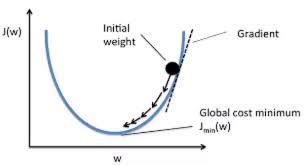
\includegraphics[width=1.0\textwidth]{gradient.png}
	\caption{LossFunktion}
	\label{fig:Bild6}
\end{figure}

Backpropagation Algorithmus wird das Verfahren genannt mit den ANN trainiert werden. Dabei wird der Gradient der Ziel Funktion bestimmt.

\subsubsection{Momentum}

Momentum hat das Ziel das Gradientenverfahren des Backpropagation Algorithmus zu beschleunigen um eine effizienter Ergebnis herbei zu führen und ein schnelleres Lernen erzielt. Definiert ist dieses durch:
\\\\
\begin{math}
v\textsubscript{t+1} =\mu v\textsubscript{t}-\epsilon\nabla$f$(\theta\textsubscript{t})
\theta\textsubscript{t+1}= \theta\textsubscript{t}+v\textsubscript{t+1}
\\\
\end{math}
\\\\
wobei $\epsilon$ $>$ 0 die Lernrate ist und $\mu$ $\in$ [0,1] das Momentum ist und $\nabla$f$(\theta\textsubscript{t}$ der Gradient von $\theta\textsubscript{t}$ ist. Je größter das Momentum desto schneller bewegt sich der Gradient abwärts. Da am Anfang eines Lernphase der Gradient üblicherweise hoch ist empfiehlt sich zunächst mit einen niedrigen Momentum zu Arbeiten da sonnst die Gefahr besteht über das globale Optimum hinüber zuschießen. Wenn nun das Training stagniert welches aus Gründe der Aufbau der Loss-Funktion zurückzuführen ist das zur nähe des globalen Optimums flache Täler entstehen welche das Trainings verlangsamen und es zu keiner Verbesserung kommt, kann man durch Momentum erzwingen größere Gradienten Sprünge einzugehen  je länger das Training voran schreitet. Und sich somit schneller zu einen globalen Optimum zu bewegen oder aber aus einen lokalen Optimum hinaus Richtung eines globalen Optimum\cite{momentum}. .


\subsubsection{Batch Normalisation}\

Wie in Kapitel \ref{sec:test} gezeigt das stochastischen Gradienten Verfahren Vorteile gegenüber des normalen Gradienten Ermittlung beim Training von KNN. Dadurch das der Input in jeden Layer abhängig von den vorherigen Layern ist können Änderungen von Werten in frühen Layern des KNN große Auswirkungen in tieferen Layern im Netzwerk haben.
Dadurch resultiert das in Trainingsabläufen die Verteilung der Gewichte in den jeweiligen Layern verlangsamt wird. Batchnormalization soll die Werteänderung von Gewichten verringen. Dieses Problem wird auch Covariance Shift genannt. Um dies zu verhindert zeigten Sergey Ioffe und Christian Szegedy \cite{batchnorm} eine Methode welche Batch Normalisation genannt wird.Je mehr Layer das Netzwerk hat desto stärker ist der Covariance Shift. Batch Normalisation besteht aus zwei Algorithmen. Algortithmus 1 verändert den eigentlichen Input von Layer n zu einen normalisierten Input y und Algorithmus 2 verändert das eigentliche Training eines Batch normalisierten Netzwerkes\cite{batchnorm}.
\\\\
\begin{algorithm}[H]
Input: Werte von x über einen Mini-Batch $B$ = \{$x\textsubscript{1},...,x\textsubscript{n}$\}\\
\begin{math}
\mu\textsubscript{$B$}\leftarrow\frac{1}{m}\displaystyle\sum_{i=1}^{m}$x$\textsuperscript{i}
\end{math}\\
\begin{math}
\sigma\textsubscript{$B$}\leftarrow\frac{1}{m}\displaystyle\sum_{i=1}^{m}($x$\textsuperscript{i} - \mu\textsubscript{$B$})\textsuperscript{2}
\end{math}\\
\begin{math}
\hat{x\textsubscript{i}}\textsubscript{$B$}\leftarrow\frac{x\textsubscript{i}-\mu\textsubscript{$B$}}{\sqrt{\sigma\textsubscript{$B$} + \epsilon}}
\end{math}\\
\begin{math}
$y$\textsubscript{i}\leftarrow\gamma\hat{x\textsubscript{i}} + \beta \equiv BN\textsubscript{$\gamma$;$\beta$}($x$\textsubscript{i})
\end{math}\\
Output: \{$y$\textsubscript{i}=BN\textsubscript{$\gamma$;$\beta$}($x$\textsubscript{i})\}
\caption{Batch Normalisierung angewand auf x über Input bei Mini-Batch  }	
\end{algorithm}

In Schritt 2 des Algorithmus 1 wird der Erwartungswert für alle Input von Mini-Batch B berechnet und In Schritt 3 die Varianze. In Schritt 3 wird nun der der normalisierte x\textsubscript{i} berechnet welche dann mit denn $\beta$ und $\gamma$ multipliziert werden. Diese Werte sind neue Gewichte im Neurnonalen Netzwerk welche während des Trainingsprozesses angepasst werden. $\epsilon$ in der Gleichung in Zeile 4 ist nur dafür da damit nicht durch 0 geteilt werden kann. In Zeile 8 - 11 werden die Inferenz Schritte beschrieben bei den der Minibatch des Trainings ersetzt wird. 

\begin{algorithm}[H]
	Input: Netzwerk N mit trainierbaren Parameter $\theta$;$\{x\textsuperscript{(k)}\}$k=1 bis 	
	\\	
	Ntr BN $\leftarrow$ N	
	\\a\\a\\a\\a\\a\\a\\a\\a\\a\\a\\

	\caption{Training mit Batch-Normalisierungs Netzwerk}	
\end{algorithm}
Schritt 1 bis 5 des Algorithmus 2 baut eigentlich nur das neuronales Netzwerk durch die Transformationen aus Algorithmus 1 um. In Schritt 6 und 7 geht es darum die Parameter $\gamma$ und $\beta$ zu trainieren. Dieses passiert mit den üblichen Backpropagation Algorithmus wären des allgemeinen Training des Netzwerkes. 

\begin{figure}[htbp] 
	\centering
	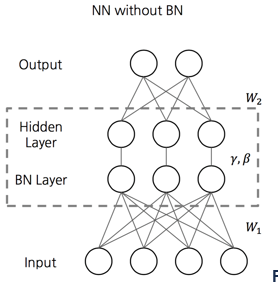
\includegraphics[width=1.0\textwidth]{batchnorm.png}
	\caption[aaaa]{Neuronales Netzwerk mit Batch Normalication Layer}
	\label{fig:Bild1}
\end{figure}

\subsubsection{Ziel-Funktion}

Die Ziel-Funktion oder auch Loss-Funktion genannt J($\theta$) muss Differenzierbar sein. Das heißt unseren Funktion f: D $\to$ R ist differenzierbar an der Stelle x\textsubscript{0}. Wenn nun $f^\prime$: x $\to$ f(x) an jeden Punkt x\textsuperscript{n} ableitbar ist, ist f differenzierbar. Die Aufgabe der Ziel-Funktion ist es zu messen wie gut unsere Model $\theta$ f*(x) approximiert. Man verwendet auch gerne den Begriff Kosten, also wie viel Kosten unser Modell erzeugt bei den lösen der zugewiesenen Aufgabe. Die Wahl welche Funktion gewählt wird ergibt sich aus der Aufgabe des KNN. Diese kann beispielsweise für Klassifikation oder Regression Aufgaben hergenommen werden. Bei Regression soll eine kontinuierlicher Variablen von $\Theta$ als Output generiert werden wohin gegen bei Klassifikationsproblemen der Output Klassen-Labels darstellen\cite{Grundlagen}. Es gibt verschiedene Ziel Funktionen im folgenden wird die Cross Entropy Loss Function vorgestellt \cite{crossentropy}. Diese kann verwendet werden um Beispielsweiße Klassikationsprobleme zu lösen. Diese ist definiert als:
\\\\
\begin{math}
\hat{q}(c\mid x)=\displaystyle\arg\min_{q(c\mid  x)}\{-\displaystyle\sum_{n}{\log q(c\textsubscript{n}\mid x\textsubscript{n})}\}
\end{math}
\\\\
Wobei  x\textsubscript{n}:n=1,...,N die Trainingsdaten sind ist und c\textsubscript{n}:n=1,...,N die mögliche Klassen. Der Output ist die Wahrscheinlichkeit zwischen 0 und 1 ob  x\textsubscript{i} $\in$ der bestimmten Klasse enthalten ist. Auch kann sie hergenommen um zu messen wie hoch die Differenz zwischen zwei Wahrscheinlichkeitsverteilungen ist.

\subsection{Datenformat}

Punktwolken sind eine Menge von N Punkten welche im Vektorraum dargestellt werden können. Jeder Punkt n $\in$ N wird durch seine (x,y,z) Koordinaten im Euklidischen Raum dargestellt. Punkte können zusätzliche Features gegeben werden wie Farbe oder Material. Es gibt unterschiedliche Dateiformate welche für die Abspeicherung von Punktwolken herangezogen werden können bespiele dafür sind PLY,STL oder OBJ. Das Polygon File Format(PLY) speichert die einzelnen Koordinaten in einer Liste diese wird Vertex List genannt. In Abb. \ref{fig:Bild13} kann eine Beispieldatei entnommen werden in der dieser Aufbau dargestellt ist. Diese kann als Menge betrachtet werden die jeweiligen Punkte sind geordnet in dieser Listen gespeichert jedoch spielt es keine Rolle für den Punktwolkencompiler bei der Visualisierung der Liste an welcher Listenposition ein jeweiliger Punkt geführt wird, die Liste wird jedes mal gleich angezeigt egal welche Permutation der einzelnen Punkte in der Liste durchgeführt wird. In Abb. \ref{fig:Bild12} kann eine visualisierte Punktwolke eines Tabakblattes entnommen werden. 

\begin{figure}[htbp] 
	\centering
	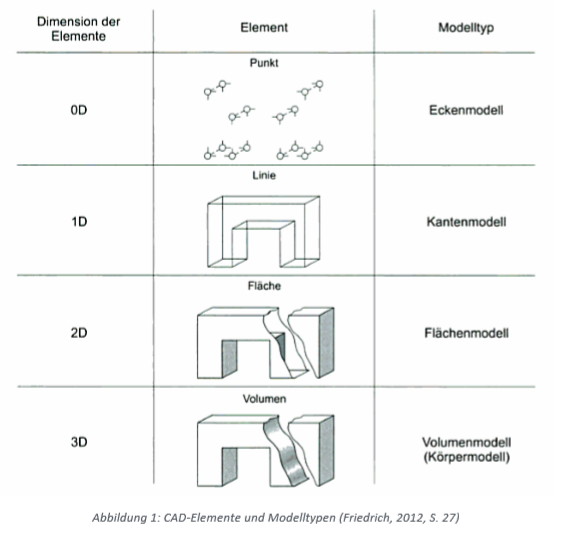
\includegraphics[width=1.0\textwidth]{datenformat.png}
	\caption{Punktwolke eines Tabakblattes}
	\label{fig:Bild12}
\end{figure}

\begin{figure}[htbp] 
	\centering
	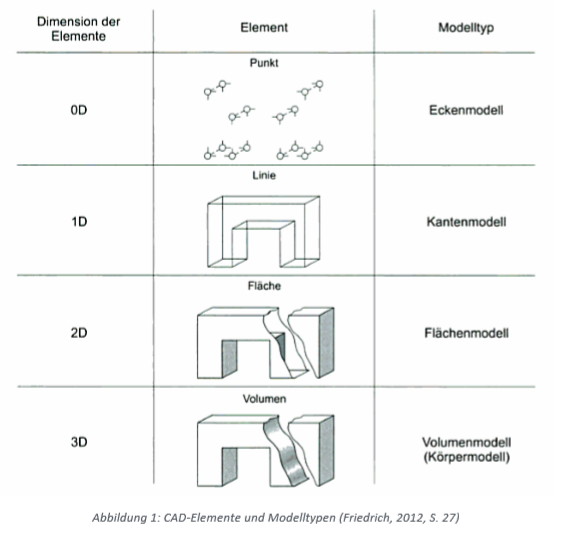
\includegraphics[width=1.0\textwidth]{datenformat.png}
	\caption{Polygon File Format}
	\label{fig:Bild13}
\end{figure}

\subsubsection{Woher stammen die Daten}
Die Daten stammen von TERRA-REF Feld Scanner von der University von Arizona Maricopa Agricultural Center and USD Arid Land Researh Station in Maricopa. Es ist der größe Feld crop scnanner. In Abb. \ref{fig:Bild13} ist dieser abgebildet. In Abb. \ref{fig:Bild14} ist der Scankopf des TERRA-REF dargestellt mit den unterschiedlichen Scanmöglichkeiten für das du scannende Objekt. 
 
\begin{figure}[htbp] 
	\centering
	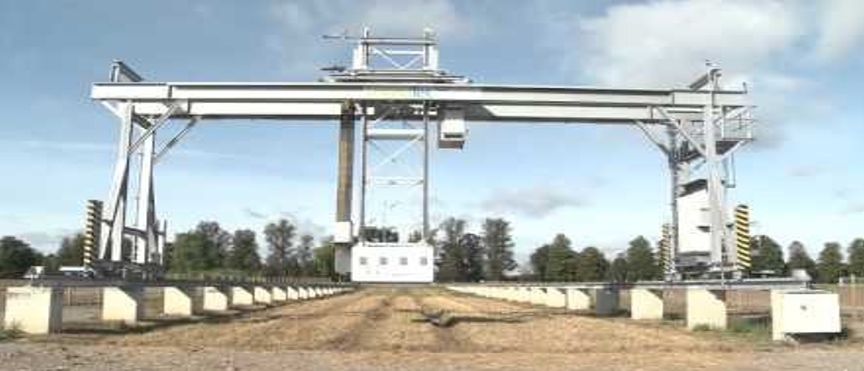
\includegraphics[width=1.0\textwidth]{lematech_1.png}
	\caption{TERRA-REF Feld Scanner}
	\label{fig:Bild13}
\end{figure}

\begin{figure}[htbp] 
	\centering
	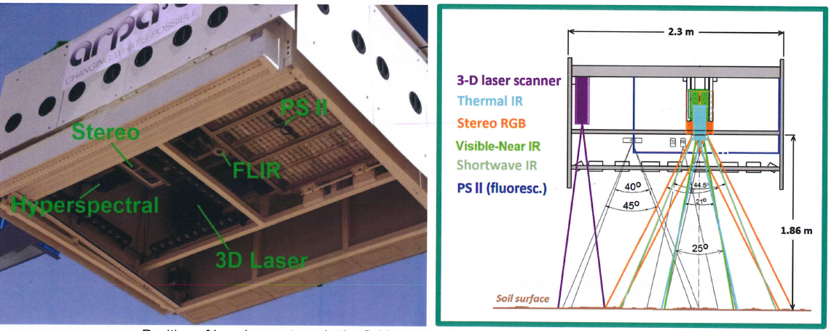
\includegraphics[width=1.0\textwidth]{lematech_2.png}
	\caption{Scankopf}
	\label{fig:Bild14}
\end{figure}

Der 3D Laser Scanner erzeugt 3D Punktwolken. Dabei werden die Objekte durch den Scanner erfasst und eine 3D Repräsentation welche durch Punkte in einen 3 Dimensionalen Koordinaten System erfasst werden können dargestellt. Dabei wird ein Laser über das zu scannende Objekt gefahren durch reflektion des Laserstrahls auf der Oberfläche des Objektes können x,y,z Koordinaten des jeweiligen Punktes auf den Objekt bestimmt werden. Durch die Sammlung eizelner Scanpunkte entsteht eine 3D-Repräsentation eines Gegenstandes. 
\subsubsection{Das Problem mit 3D-Data bei Machine Learning Ansätzen}
Vergleicht man 3D-Data auf ihre Dimensionalität mit anderen Datenformaten wie Bild,- , Audio ,- Textdateien steigt der Informationsgehalt und dadurch die Komplexität für das Anwenden von Maschine Learning Algorithmen enorm. Besonders bei Nicht-Euklidischen 3D-Daten wie Punktwolken deren keine Struktur zu Grunde liegt ist dieses gegeben \cite{3dprob}.
\\
Wie im Kapitel "Woher stammen die daten " gezeigt, sind Punktwolken als Menge gespeichert in denen keine Relation untereinander besteht, dass heißt es ist für den Punktwolkencompiler nicht von Relevanz auf welchen Platz die einzelnen Punkte abgespeichert werden, die Punktwolke wird egal in welcher Permutation der einzelnen Punkte abgespeichert, immer gleich angezeigt. Vergleicht man nun ein Bild mit 512 Pixeln und 3 RGB-Farbkanälen ist einer Dimension von 391680 erreicht. Vergleichen wir nun das mit einer Punktwolke in einen 125 cm \textsubscript{3} großen Bereich. Da die einzelen Koordianten eines Punktes als Rationale Zahlen dargestellt wird und rationalen Zahlen abzählbar Unendlich ist unser Suchraum "unendlichzeichen " groß. Dies führt zu einen erheblichen mehr Aufwand für Machine Learning Ansätzen wie Deep Learning für Punktwolken.
\\
Ein weitere Schwierigkeit die für Deep Learning mit Punktwolken ist, dass die aus Kapitel Convolutional Neural Network beschrieben Convolutionel-Layer einen großen Beitrag bei den Fortschritt von Deep Learning gebracht hat. Da sie helfen die Strukturen von strukturierten Daten zu lernen und den latenten Raum zu entdecken. Da jedoch Pointclouds unstrukturiert sind hilft es nicht diese Tools bei Punktwolken einzusetzen\cite{3dgan}. 

\subsection{Convolution Neural Networks}

Convolution Neural Netzworks(CNN) sind eine besondere Art von künstlichen neuronalen Netzwerken, sie sind dafür konzipiert auf Datensätzen zu arbeiten welche in eine Matrix Form gebracht worden sind. Der Input eines CNN können beispielsweise Bilder sein welche durch die Matrix A =
$
\begin{bmatrix}
a_1	& a_1	& \dots	 & a_n     \\
b_1	& b_2 	& \dots  & b_n	  \\
\vdots	& n_n 	& \ddots & \vdots \\
x_1 	& x_2 & x_3	 & x_n
\end{bmatrix}
$
\\\\dargestellt werden. Jedes Element x\textsubscript{ij} stellt einen Pixel eines Bildes da, wobei x\textsubscript{n} $\in$ [0,255] . Die Matrix A\textsuperscript{w$\cdot$b$\cdot$c} stellt w$\cdot$b$\cdot$c = N dimensionale Matrix da. Wobei w die Länge und b Breite des Bildes entspricht. c sind die Farbspektren eines Bildes und sind in einen RGB-Farbraum 3 beziehungsweiße in einen schwarz-weiß Bild 1. Nachdem  der Input eines CNN definiert ist kommt nun der Aufbau. CNN setzen sich aus mehrere Schichten von Convolution Layern zusammen. Ein Netzwerk kann mehrere N-Layer haben. Wobei jeder Layer aus mehreren Convolution oder auch Kernels genannt, zusammengesetzt ist. Ein Aufbau kann aus Abbildung \ref{fig:Bild2} entnommen werden\cite{Grundlagen}.

\begin{figure}[htbp] 
	\centering
	\includegraphics[width=1.0\textwidth]{convol.png}
	\caption{Convolutional Neural Network}
	\label{fig:Bild2}
\end{figure}

Die Kernels, also die einzelnen Filter, von den jeder der N-Layer k besitzt sind K\textsuperscript{n$\cdot$n} Matrizen jedes k\textsubscript{ij} in einem Filter einspricht einen aus der üblichen Neuronalen Netzwerk Architektur bekannten Gewichte. Diese Gewichte werden dann durch den Backprobagation-Algorithmus in der Trainingsphase des Netzwerkes angepasst um den Verlust der Loss-Funktion durch bestimmten des Gradianten zu minimieren. Das durch die Abbildung \ref{fig:Bild2} dargestellte Subsampling ist der Output aus den Convolutional Layern\cite{Grundlagen}. 

Da Input und Kernel unterschiedliche Größen haben und man den gesamten Input mit den Kernel abdecken möchte, bewegt sich der Filter um s Position auf den Input und führt erneut einen Berechnungschritt durch. Dieser Vorgang wird Stride genannt. An jeder Position wird das Produkt von jeden x\textsubscript{ij} des Input und k\textsubscript{ij} des Kernel durchgeführt.  Anschließend werden alle Produkte aufsummiert. In Abbildung \ref{fig:Bild3} ist dieser Vorgang verdeutlicht. Zusätzlich gibt es die Möglichkeit für das sogenannte Zero Padding P. Dabei werden mehrere 0 um die Input Feature Map, am Anfang und Ende der Axen anfügt. Dies ist notwendig wenn Kernel und Input Größe nicht kompatible zueinander sind. Die Anzahl der möglichen Positionen ergeben sich aus Kernel Größe und den Input des jeweiligen Kernel sowie des Strides. Die Output Größ W kann berechnet werden durch W = (W-F+2P)/s+1. Wobei F für die Größe des Kernel steht \cite{conv}.

\begin{figure}
	\centering
	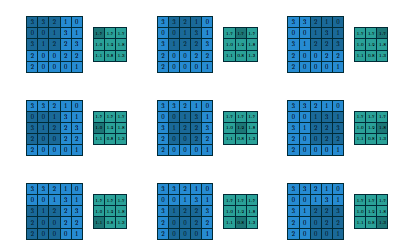
\includegraphics[width=0.8\textwidth]{conv.png}
	\caption{Convolution Beispiel}
	\label{fig:Bild3}
\end{figure}

Um  besser zu verstehen welche Auswirkungen die Anzahl der Kernels in Layer n auf die Größe des Outputs von n und die Anzahl der Kernels in Layer n+1 für den nächsten Layer haben, wird ein Beispiel aufgezeigt. Der erste Layer hat 20 Kernels mit der Größe 7x7 und Stride 1. Der Input A für einen Kernel K ist ein 28x28 Matrix. Der Output aus diesen Filter sind 20 22X22 Feature Maps. Würde der Input ein 28x28x3 Bild mit 3 RGB Channels sein, der Output 60 22x22 Feature Maps. Allgemein kann Convolution Layer als Supsampling gesehen werden und Stride gibt an wieviele Dimensionen bei diesen Prozess pro Convolution Layer entfernt werden soll. Der letzte Layer ist ein fully-connected Layer welcher den typischen Anforderungen von ANN entspricht \cite{conv}.  
\\
Transposed Convolution, auch genannt Fractionally Strided Convolution oder Deconvolution ist eine Umkehrfunktion von der üblichen Convolution. Es verwendet die gleichen Variablen wie Convolution. Dabei wird ein Kernel K mit der Größe N x N definiert der Input I mit der Größe N x N und Stride s = 1. Deconvolution kann wie Convolution angesehen werden mit  Zero Padding auf dem Input.  Das in Abbildung \ref{fig:Bild4} gezeigte Beispiel zeigt einen deconvolution Vorgang mit eine 3x3 Kernel über einen 4x4 Input. Dies ist gleich mit einen Convolution Schritt mit einen 3x3 kernel auf einen 2x2 Input und einer 2x2 Zero Padding Grenze. Convolution ist Supsampling und mit Deconvolution wird Upsampling betrieben. Durch diesen Schritt kommt es zu einer Dimensionserhöhung des Inputs. Die Gewichte der Kernels bestimmen wie der Input transfomiert wird. Durch mehrere Schichten von Deconvolution Layer kann von einer Input Größe NxN auf eine Output Größe KxK, wobei K $>$ N mit Abhängigkeit von Kernel und Stride abgebildet werden\cite{conv}. 

\begin{figure}[htbp] 
	\centering
	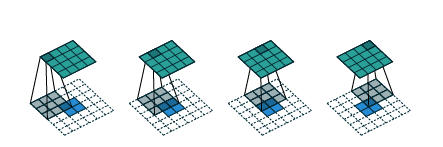
\includegraphics[width=1.0\textwidth]{decon.png}
	\caption{Deconvolution Beispiel}
	\label{fig:Bild4}
\end{figure}
\newpage

\subsection{Autoencoder}

Autoencoder gehören zu den generativen Modellen im Bereich des Machine Learnings. Generative Modelle haben das Ziel eine Wahrscheinlichkeitsverteilungen zu erlernen. Anschließend kann diese als ein Modell genutzt werden und Samples aus dieser zu erzeugen. Die Modelle können dabei beispielsweise auf ANN oder Markov Chains trainiert werden\cite{Grundlagen}. Im folgenden liegt der Fokus auf ANNs. Allgemein gehalten können jegliche Typen von Daten wie Text, Bild oder Audiodateien für generative Modelle herangezogen werden. Es gibt unterschiedliche Typen von generativen Modellen, welche sich vom Aufbau des Neuronalen Netzwerk und der Zielfunktion unterscheiden. Beispiele dafür sind Boltzmann Maschine, Autoencoder oder Deep Belief Networks\cite{Grundlagen}.
\\
Autoencoder sind ein andere Art von Model aus den Bereich der generativen Modelle. Ihre Aufgabe besteht darin einen Input zu komprimieren und aus der komprimierten Information den Input wieder herzustellen. Die Technik auf welche Autoencoder zurückgreifen nennt sich Dimensionreduction. Dabei werden die Dimension der Daten so reduziert und Informationen bei zu behalten welche als relevant gelten. Diese Technik finden auch in anderen Machine Learning Anwendung wie in beispielsweise der Principale component anaysis(PCA) Anwendung.  Ein Autoencoder besteht aus 2 Bestandteilen. Erstens ein Encoder e parametrisiert mit $\phi$ welcher einen Input x $\in$ von $x\textsuperscript{i}$ wo x ein Vektor der länge i ist und damit die Input Dimension bestimmt. Dieser wird durch den Encoder auf einen Vektor $z\textsuperscript{k}$ abgebildet wobei k<i ist.  Zweitens der Decoder d parametrisiert durch  $\theta$ bekommt als Input t$z\textsuperscript{k}$ und bildet z auf $x\textsuperscript{l}$ ab wobei l = i. Und somit die gleiche Dimension wie der Input. Aufgabe ist es nun das der Encoder den Input z so gut komprimiert das der  Encoder es schafft das x $\thickapprox$ z. Eine grafische Darstellung kann aus Abb. $\ref{fig:Bild8}$ entnommen werden. 
\\
Die Paramter $\phi$ und $\theta$ werden durch durch den in Kapitel "Backprobagation Algorithmus" erlernt. Und können beispielsweise durch Fully-Connected-Layer, Convolutional-Layer oder Deconvolutional-Layer modelliert werden. Eine Metrik um zu messen wie das Model seine Aufgabe erfüllt könnte Beispielsweiße Cross-Entropy Funktionen sein welche schon in Kapitel"" vorgestellt worden ist. Weitere spezifische Zielfunktionen für Autoencoder welche mit 3D-Daten arbeiten werden nun vorgestellt.

\begin{figure}[htbp] 
	\centering
	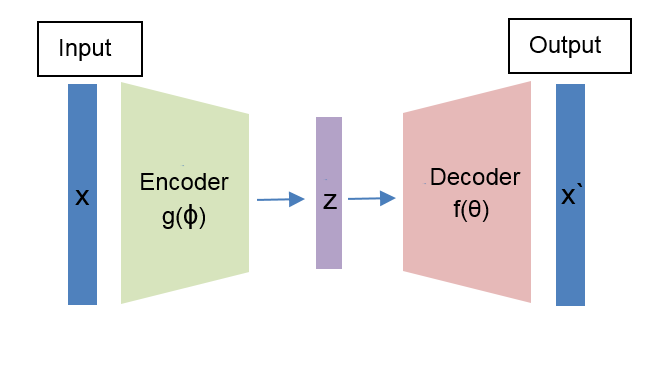
\includegraphics[width=1.0\textwidth]{autoencoder.png}
	\caption{autoencoder}
	\label{fig:Bild8}
\end{figure}

Bei Punktwolken als Datentyp erzielt die  Cross-Entropy-Zielfunktion keine gute Ergebnisse da diese Invariant zu ihrer Permutation sind\cite{3dgan}. Das heißt ändere ich die Anordnung meiner einzelnen Punkte in mein Set bleibt das Ergebnis unverändert.  Deshalb kann auf die Cross-Entropy-Zielfunktion übliche Zielfunktionen welche für strukturierte Daten wie Bilder verwendet werden nicht zurück gegriffen. Das Problem dabei besteht das zwischen zwei unterschiedliche Sets von Punkten heraus zu finden wie hoch die Diskrepanz zwischen den beiden Sets ist um sie dahingehen durch Backpropagation zu optimieren diesen Abstand zu verringern. In Abbildung \ref{fig:Bild1} ist dieser Prozess dargestellt. 
 http://graphics.stanford.edu/courses/cs468-17-spring/LectureSlides/L14%20-%203d%20deep%20learning%20on%20point%20cloud%20representation%20(analysis).pdf

Eine Möglichkeit speziell für Autoencoder welche mit Punktwolken arbeiten, ist die Earth Mover Distance(EMD). Bei dieser sind X\textsuperscript{1} und X\textsuperscript{2} zwei Punktwolken mit jeweils x\textsuperscript{n} definierten Punkten\cite{autoencoderloss}. Definiert ist sie durch die Funktion:

\begin{math}
d\textsuperscript{EMD}=\min_{\theta : X\textsubscript{1}\rightarrow X\textsubscript{2}}  \sum_{x\in X\textsubscript{1}} || x - \theta(x)\textsubscript{2} wobei \theta: X\textsubscript{1} \rightarrow X\textsubscript{2} bijektiv ist 
\end{math}

Grafisch kann man sich die Berechnung wie in Abb. \ref{fig:Bild9} darstellen. Ein Punkt von x\textsuperscript{n} $\in$ X\textsuperscript{1} wird den nähsten Punkt y\textsuperscript{n} $\in$  X\textsuperscript{2} zugewiesen. Wobei die Distanz durch die Euklidische Distanz der jeweiligen Punkte ermittelt wird.
 
\begin{figure}[htbp] 
	\centering
	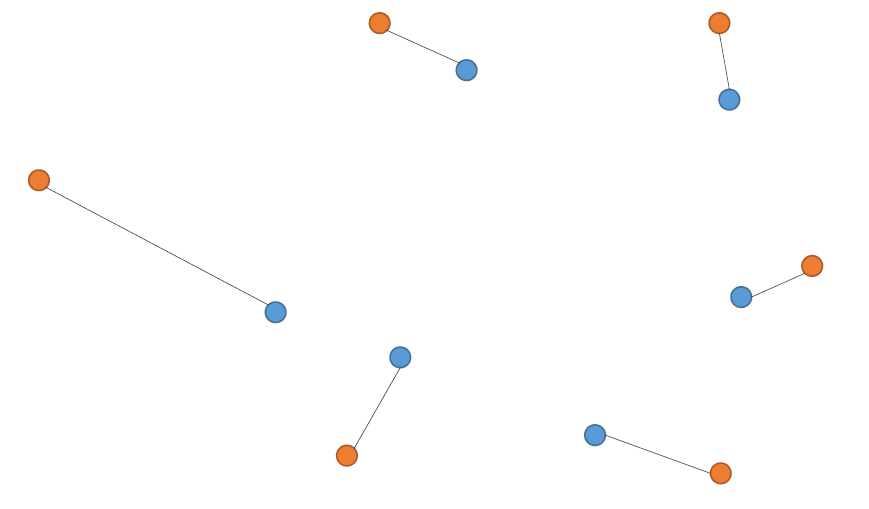
\includegraphics[width=1.0\textwidth]{emd.png}
	\caption{Earth Mover Distance}
	\label{fig:Bild9}
\end{figure}
		
Eine weitere Möglichkeit ist die Chamfer Distance(CD). Wie auch zuvor sind  X\textsuperscript{1} und X\textsuperscript{2} zwei Punktwolken mit jeweils x\textsuperscript{n} definierten Punkten\cite{autoencoderloss}. Definiert ist sie durch die Funktion:

\begin{math}
d\textsuperscript{CD}(X\textsubscript{1},X\textsubscript{2})=\sum_{x\in X\textsuperscript{1}} \min_{y \in X\textsuperscript{2}}||x-y|| + \sum_{y\in X\textsuperscript{2}} \min_{x \in X\textsuperscript{2}}||x-y||
\end{math}

Der Unterschied ergibt sich zwischen den beiden das bei der EMD von der Ausgangswolke die Punkte zu der anderen jeweils optimiert werden. Wohingegen bei der CD die Distanzen von und zu der Ausgangspunktwolke berechnet werden. Dies geht aus den Abb. \ref{fig:Bild10} hinaus in welche die Distanzberechnung der einzelnen Punkte dargestellt wird\cite{autoencoderloss}.

\begin{figure}[htbp] 
	\centering
	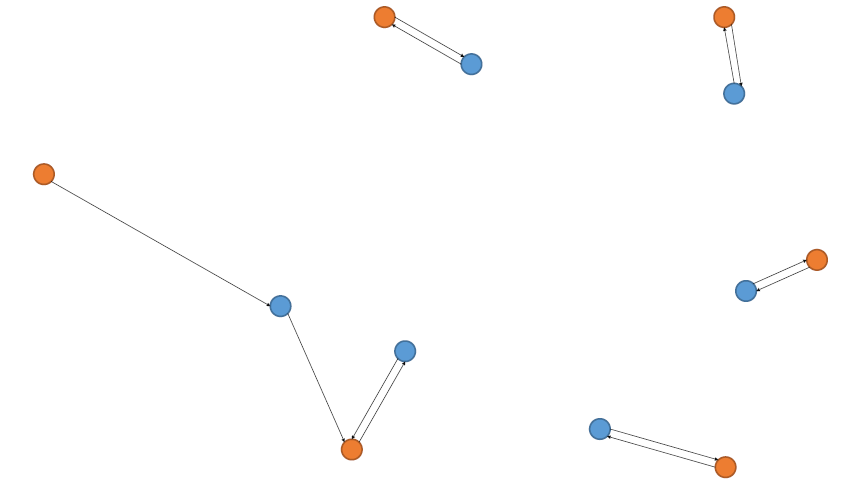
\includegraphics[width=1.0\textwidth]{chamfer.png}
	\caption{Chamfer Distance}
	\label{fig:Bild10}
\end{figure} 

\subsection{Generative Adversarial Network}

In Abbildung \ref{fig:Bild1} ist dieser Prozess dargestellt. Diese Modelle versuchen dann die diese Cost Funktion  
\\
\\
\begin{math}
KL(P\textsubscript{r}|| P\textsubscript{g}])=\int_x P\textsubscript{r}log\frac{P\textsubscript{r}}{P\textsubscript{g}}dx                     
\end{math}
\\
\\
zu minimieren. Wenn nun beide Verteilungen P\textsubscript{r} = P\textsubscript{g} sind, hat das Model sein Minimum Loss erreicht und $\Theta$ muss nicht mehr angepasst werden. Interessant wird es, wenn P\textsubscript{r} $\ne$ P\textsubscript{g}.
Wenn  P\textsubscript{r} $>$ P\textsubscript{g} führt, das dazu dass das Integral schnell gegen unendlich konvergiert. Was dazuführt, das hohe Kosten entstehen wenn die  Verteilung von generativen Modell erzeugt, nicht die Daten abdeckt. Wenn nun  P\textsubscript{r} $<$ P\textsubscript{g} ist, dann bedeutet das, dass x eine niedrige Wahrscheinlichkeit hat aus unseren Trainingsdaten zu kommen aber eine hohe Wahrscheinlichkeit von den Generator erzeugt zu werden. Dann würde sich die KL gegen 0 konvergieren. Was zur Folge hat, dass der Generator Falsch ausschauende Daten geniert aber keine Kosten dafür erzeugt werden und im Umkehrschluss es zu keinen Veränderungen unseren $\Theta$ kommt. Man vermutet das dies der Grund für die Problematiken von generativen Modellen wie Autoencoder und CO sind. Dies ist aber noch kein abgeschlossenen Problem und wird weiterhin erforscht\cite{improvingan}.
Unter GAN werden wir auf dieses Problem erneut aufgreifen und es wird gezeigt inwiefern sich GAN dieses Problem angeht. Generative Modelle gehören zu einem Bereich des unüberwachten Lernens, da keine Labels für die Trainingsdaten gebraucht werden. Probleme welche diese Modelle haben sind beispielsweise, dass Autoencoder zwar mit wenig Trainingsaufwand trainiert werden können jedoch sind die generierten Bilder sehr trüb. Allgemein haben Autoencoder und Co. Vorteile  im Lernen des latenten Raums von Objektlassen, weisen aber Probleme beim Generieren von neuen Daten auf. Da gezeigt wurde das im Deep Learning Bereich die discrimativen Modelle mit Zunahme der Daten stark an Leistung zunehmen. Und GANs Stärke in der Datengeneration in guter Qualität liegt. Kann es seine Vorteil gegenüber den anderen Modellen ausspielen\cite{improving}


In den letzten Jahren konnte sich das GAN als best practice Ansatz bei den generativen Modellen herausarbeiten was Performancegründe bei der Trainierbarkeit und Qualität der generierbaren Daten zu Grunde liegt\cite{Grundlagen}. 
Die Modelle arbeiten nach der Maximum Likelihood Schätzverfahren(ML-Schätzer) in dem die Parameter $\theta$ dahingegen angepasst werden, dass die unsere beobachtetet Daten am ehesten passen. Man kann ML-Schätzer als Kulback-Leibler(KL) Divergenz darstellen und das generative Modelle das Ziel haben die KL Divergenz zwischen den Trainingsdaten P\textsubscript{r} und den generierten Daten P\textsubscript{g} zu minimieren.

Ein GAN besteht besteht aus zwei KNN, dem Discriminator D und dem Generator G. Das Ziel des G ist es, Daten x zu erzeugen, welche nicht von Trainingsdaten y unterschieden werden können. Dabei wird eine vorangegangene Input Noise Variable p\textsubscript{z}(z) verwendet, welche eine Abbildung zum Datenraum G(z;$\Phi$\textsubscript{g}) herstellt. Dabei sind $\Phi$\textsubscript{g} die Gewichte des neuronalen Netzwerkes von G. Der Discriminator hat die Aufgabe zu unterscheiden, ob der jeweilige Datensatz von G erzeugt wurde und somit ein fake Datensatz ist, oder von Trainingsdaten y stammt\cite{goodfellow2014}. Die Zusammensetzung zwischen den beiden Netzwerken kann aus Abbildung \ref{fig:Bild20} entnommen werden.
\\
\begin{figure}[htbp] 
	\centering
	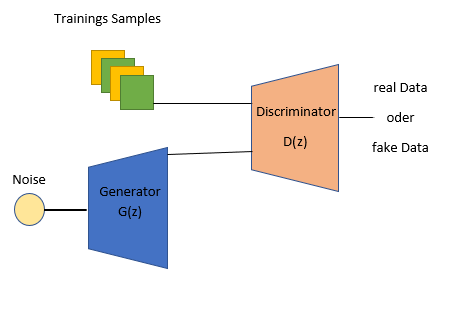
\includegraphics[width=1.0\textwidth]{GAN_GRUNDAUFBAU.png}
	\caption{Generativ Adverserial Network}
	\label{fig:Bild20}
\end{figure}

Der Discriminator ist definiert durch D(x;$\Phi$\textsubscript{d}). Wobei $\Phi$\textsubscript{d} die Gewichte des Descriminators sind und D(x) die Wahrscheinlichkeit ist, dass x von den Trainingsdaten stammt und nicht von p\textsubscript{g}. Die Wahrscheinlichkeitsverteilung für unsere Trainingsdaten ist p\textsubscript{r}.  Im Training werden dann $\Phi$\textsubscript{d} so angepasst, dass die Wahrscheinlichkeit Trainingsbeispiele richtig zu klassifizieren maximiert wird. Und $\Phi$\textsubscript{g} wird dahingehen trainiert die Wahrscheinlichkeit zu minimieren, so dass D erkennt dass Trainingsdatensatz x von G erzeugt wurde. Mathematisch ausgedrückt durch log(1 - D(G(z))). Die gesamte Loss-Funktion des vanilla GAN ist definiert als
\\\\
\begin{math}
min\textsubscript{G} max\textsubscript{D}V(D,G)=E\textsubscript{x$\sim$p\textsubscript{data}(x)}[logD(x)]  + E\textsubscript{z$\sim$p\textsubscript{z}(z)}[log(1-D(G(z))]
\\\\             
\end{math}
diese beschreibt ein Minmax Spiel zwischen G und D. Welches das globale Optimum erreicht hat wenn p\textsubscript{g} = p\textsubscript{r}. Das heißt, wenn die Datenverteilung, welche von G erzeugt wird, gleich der unserer Trainingsdaten ist\cite{goodfellow2014}. Das Training erfolgt durch den folgenden Algorithmus:
\\
\begin{algorithm}[H]
	\For{Anzahl von Training Iterationen}{\For{k Schritte}{$\bullet$Sample minibatch von m noise  Samples z\textsuperscript{(1)},...,z\textsuperscript{(m)}von noise p\textsubscript{g}(z)\\
	$\bullet$ Sample minibatch von m Beispielen x\textsuperscript{(1)},...,x\textsuperscript{(m)}von Daten Generationsverteilung p\textsubscript{data}(x)\\
    $\bullet$ Update den Discriminator zum aufsteigenden stochastischen Gradianten:\\
\begin{math}
\nabla\textsubscript{$\Phi$\textsubscript{d}}\frac{1}{m}\sum_{i=1}^{m}[logD(x\textsuperscript{(i)})+log(1-D(G(z\textsuperscript{(i)})))]
 \end{math}

}$\bullet$ Sample minibatch von m noise Samples z\textsuperscript{(1)},...,z\textsuperscript{(m)} von noise p\textsubscript{g}(z)\\$\bullet$ Update den Generator mit den absteigenden stochastischen Gradianten: \\\begin{math} 
\nabla\textsubscript{$\Phi$\textsubscript{g}}\frac{1}{m}\sum_{i=1}^{m}log(1-D(G(z\textsuperscript{(i)})))\end{math}}
		\caption{Minibatch stochastic gradient descent Training für Generative Adversarial Networks. Die Anzahl der Schritte welche auf den Discriminator angewendet wird ist k }	
\end{algorithm}

Beim Training wird ein stochastischer Minibatch von mehren Trainingsdaten gleichzeitig erstellt. Dies soll dabei helfen, dass der Generator sich nicht auf bestimmte Gewichte fest fährt und auf Trainingssätze kollabiert. So weisen die erzeugten Daten mehr Variationen auf \cite{improvingan}. D wird zunächst in einer inneren Schleife auf n Trainingsätzen trainiert, womit man Overfitting von D vermeiden will, was zur Folge hätte, dass D nur den Trainingsdatensatz kopieren würde. Deshalb wird k mal D optimiert und ein mal G in der äußeren Schleife. 
\\\\
Ein möglicher Aufbau von GAN wird in Abbildung \ref{fig:Bild21} dargestellt. Dies ist das sogenannte Deep Convolution GAN(DC GAN), welches dafür konzipiert wurde auf Bilddaten zu arbeiten. Dabei besteht der Generator aus mehren Schichten von Deconvolution Layern. Welche den Input Noise Variable p\textsubscript{z}(z) auf y abbildet. D besteht aus mehren Schichten von Convolution Layern und bekommt als Input die Trainingsdaten, oder die von G erzeugten Y, und entscheidet über die Klassifikation\cite{dcgan}.

\begin{figure}[htbp] 
	\centering
	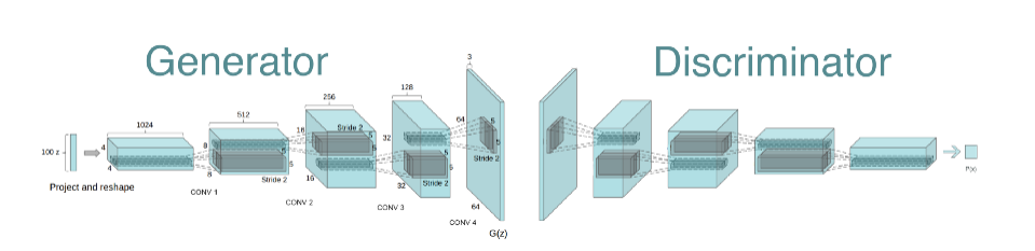
\includegraphics[width=1.0\textwidth]{dcgan1.png}
	\caption{Deep Convolutional GAN}
	\label{fig:Bild21}
\end{figure}

Wie unter Generativen Modellen gezeigt wurde kann das asymmetrische Verhalten der KV Divergenz zu schlechten Trainingsergebnissen führen. Goodfellow \cite{goodfellow2014} zeigte, dass sich die MinMax Loss-Funktion des GAN auch als Jensen-Shannon Divergenz(JS Divergenz) darstellen lässt. Diese ist definiert als\\

\begin{math} D\textsubscript{JS}(P\textsubscript{r}|| P\textsubscript{g}])=\frac{1}{2}D\textsubscript{KL}(P\textsubscript{r}|| \frac{P\textsubscript{g}+P\textsubscript{r}}{2}])+D\textsubscript{KL}(P\textsubscript{q}|| \frac{P\textsubscript{g}+P\textsubscript{r}}{2}])  
\end{math}
\\

wobei P\textsubscript{r} die Wahrscheinlichkeitsverteilung der Trainingsdaten ist und P\textsubscript{g} die des Generators. Huzár \cite{sha} zeigte, dass durch das symmetrische Verhalten der JS Divergenz ein potentiell besseres Trainingsergebnis entstehen kann, im Vergleich zu der KL Divergenz. Damit zeigte er weshalb GANs im Vorteil gegenüber anderen generativen Modellen sind. Abbildung \ref{fig:Bild21} veranschaulicht dieses Konzept. Der linke Graph zeigt 2 Normal Verteilungen. In der Mitte wird die KV Divergenz der beiden Normal Verteilungen dargestellt.  Rechts ist die JS Divergenz der Beiden dargestellt. Man sieht sehr gut das asymmetrische Verhalten der KV und das symmetrische der JS. Dadurch lassen sich aussagekräftigere Gradianten bestimmen, welche zum Optimieren von D und G benötigt werden\cite{sha}. 
 
\begin{figure}
	\centering
	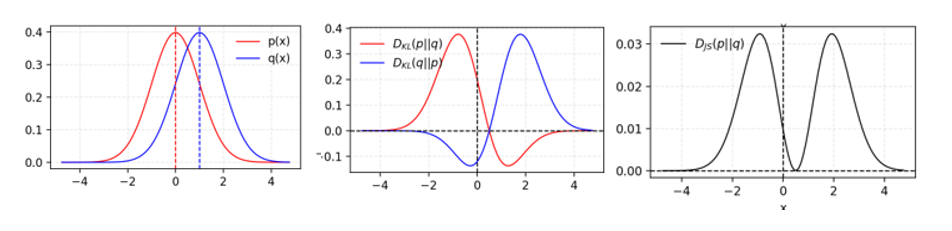
\includegraphics[width=1.0\linewidth]{KLdiv}
	\caption{KL Divergenz und JS Divergenz}
	\label{fig:Bild21}
\end{figure}

\subsubsection{Probleme mit Generative Adverserial Networks}

Wie auch anderen generativen Modelle haben auch GANs noch Schwächen bezüglich der Trainingsabläufe und der Qualität der generierten Daten. Im Folgenden wird auf einige Probleme eingegangen welche im darauffolgenden Kapitel Lösungsansätze aufgezeigt werden. 

\begin{description}	

\item[Equilibrium]
D und G betreiben ein MinMax Spiel. Beide versuchen das Nash Equilibrium zu finden. Dies ist der bestmögliche Endpunkt in einen nicht kooperativen Spiel. Wie in dem Fall von GAN wäre das wenn  p\textsubscript{g} = p\textsubscript{r}. Es wurde gezeigt, dass das Erreichen dieses Punktes sehr schwierig ist, da durch die Updates der Gewichte mit den Gradianten der Loss-Funktion starke Schwingungen der Funktion enstehen können. Dies kann zur Instabilität für das laufende Training führen \cite{improvingan}.   
\\
\item[Vanishing gradient]
Dies beschreibt das Problem, wenn D perfekt trainiert ist mit  D(x) = 1, $\forall \in p\textsubscript{r}$ und D(x)=0 $\forall x \in p \textsubscript{g}$. Die Loss-Funktion würde in diesem Fall auf 0 fallen und es gäbe keinen Gradianten, für den die Gewichte von G angepasst werden können. Dies verlangsamt den Trainingsprozess bis hin zu einem kompletten Stopp des Trainings. Würde D zu schlechten trainiert mit  D(x) = 0, $\forall \in p\textsubscript{r}$ und D(x)=1 $\forall x \in p \textsubscript{g}$. Bekommt G kein Feedback über seine Leistung bei der Datengeneration hat er keine Möglichkeit p\textsubscript{r} zu erlernen \cite{improvingan}.
\\
\item[Mode Collapse]
Während des Trainings von GAN kann es dazu kommen, dass der Generator möglicherweise auf eine Einstellung seiner Gewichte fixiert wird und es zu einem sogenannten Mode Collapse führt. Was zur Folge hat, dass der Generator sehr ähnliche Samples produziert \cite{wasserstein}.
\\
\item[Keine aussagegräftigen Evaluations Metriken]
Die Loss Funktion der GANs liefert keine aussagekräftigen Evaluationsmöglichkeit über den Fortschritt des Trainings. Bei  discriminativen Modellen im üblichen Maschine Learning besteht die Möglichkeit Validierungsdatensätze zu verwenden und an diesen die Genauigkeit des Modells zu testen. Diese Möglichkeit besteht bei GANs nicht\cite{metrics}.
\end{description}
\newpage

\subsubsection{Lösungsansätze für Generative Adverserial Networks Probleme}

Nun werden einige Techniken aufgezeigt, welche die unter Abschnitt Probleme mit GAN genannten Schwierigkeiten angehen und zu einem effizienteren Training führen, damit eine schnellere Konvergenz während des Trainings erreicht wird.
\begin{description}
\item[Feature matching]
Dies soll die Instabilität von GANS verbessern und gegen das Problem des Vanishing Gradient angehen. G bekommt eine neue Loss-Funktion und ersetzt die des üblichen Vanilla GAN. Diese soll G davon abhalten, sich an D über zu trainieren und sich zu sehr darauf zu fokussieren, D zu täuschen und gleichzeitig auch versuchen die Datenverteilung der Trainingsdaten abzudecken\cite{improvingan}.\\

\item[Minibatch discrimination] Um das Problem des Mode Collapse zu umgehen, so dass es nicht zu einem Festfahren der Gewichten von G kommt, wird beim Trainieren die Nähe von den Trainingsdatenpunkten gemessen. Anschließend wird die Summe über der Differenz aller Trainingspunkte genommen und dem Discriminator als zusätzlicher Input beim Training hinzugegeben \cite{improvingan}.\\

\item[Historical Averaging] 
Beim Training werden die Gewichte von G und D aufgezeichnet und je Trainingsschritt i verglichen. Anschließend wird an die Lossfunktion je Trainingschritt die Veränderung zu i-1 an die Loss-Funktion addiert. Damit wird eine zu starke Veränderung bei den jeweiligen Trainingsschritten bestraft und soll gegen ein Model Collapse helfen \cite{improvingan}.\\

\item[One-sided Label Smoothing]
Die üblichen Label für den Trainingsdurchlauf von 1 und 0 werden durch die Werte 0.9 und 0.1 ersetzt. Dies führt zu besseren Trainingsergebnissen. Es gibt derzeit nur empirische Belege für den Erfolg, jedoch nicht weshalb diese Technik besser funktioniert\cite{improvingan}.\\

\item[Adding Noises] 
Noise an den Input von D zu hängen kann gegen das Problem des Vanishing gradienten helfen und das Training verbessern\cite{improvingan}.\\

\item[Use Better Metric of Distribution Similarity] 
Die JS Divergenz von vanilla GAN sorgt für bessere Trainingsergebnisse im Vergleich zu der KL Divergenz von anderen generativen Modelle. Jedoch weißt die JS immernoch Probleme auf.  Es wird vorgeschlagen diese durch die Wasserstein Metric zu ersetzen, da diese bessere Ergebnisse bei disjunkten Wahrscheinlichkeitsverteilungen liefern kann\cite{improvingan}.\\

\item[Wasserstein-GAN]

Die Wasserstein Metric oder auch Earth Mover Distance genannt mist die Minimum Kosten welche enstehen wenn man Daten von der Datenverteilung $/alpha$ zur Datenverteilung $/omega$ überträgt werden. Es wird oft auch von Masse oder Fläche gesprochen, welche von $/alpha$ zu $/omega$ getragen wird. 

\begin{math} 
$
W(p\textsubscript{r},p\textsubscript{g})=$\inf_{\gamma\sim\prod(P\textsubscript{r},P\textsubscript{g})}$E\textsubscript{(x,y)$\sim\gamma$}[$\parallel$x - y$\parallel$]
$
\end{math}

p\textsubscript{r} steht für die reale Datenverteilung zu welcher uns Daten zur Verfügung stehen und p\textsubscript{g} steht die generierte Datenverteilung. Dabei wird nun das Infinum von allen Möglichen Transportplänen $\gamma$ welche in $\prod$ enthalten sind ausgewählt. Vorteile sind unter anderem, dass der Gradiant gleichmäßiger ist und das WGAN lernt besser auch wenn der Generator schlechtere Daten erzeugt im Vergleich zum üblichen GAN.
Durch die Kantorovich-Rubinstein Methode kann die Wasserstein-Distanz umgeformt werden in:
\begin{math} 
$
W(p\textsubscript{r},p\textsubscript{$\theta$})=$\sup_{\parallel f \parallel \textsubscript{L}\leq 1}$ E\textsubscript{x$\sim$P\textsubscript{r}}[f(x)] - E\textsubscript{x$\sim$P\textsubscript{$\theta$}}[f(x)]
$
\end{math}

Durch diese Umformung ist es nun Möglich das GAN so zu gestalten durch die Funktion zu erlernen. Dabei übernimmt der Discriminator nun die Aufgabe eines Critic welcher nun nicht mehr 0 oder 1 für Fake oder Real ausgibt sondern einen Score welcher angibt wieviel Masse von der P\textsubscript{$\theta$} umverteilt werden muss damit der Generator bessere Ergebnisse liefert. 
EVTL lern algortithmus hier:
\end{description}

\subsection{Conditional-GAN}

Conditional-GAN(C-GAN) ist eine Modifikation des ursprünglichen GAN von Goodfellow, welches erlaubt bedingte Wahrscheinlichkeiten in Datensätze zu erlernen. Das heißt zusätzliche Informationen in den Lernprozess einzuspeisen um den Output zu modifizieren. Im ursprünglichen GAN gibt es keine Möglichkeit auf den Output des Generators Einfluss zu nehmen. Dabei wird das Modell so verändert das eine zusätzliche Information y als Input in den Discriminator und Generator zugefügt wird. Dabei kann y jegliche Information sein wie Label, Bilddaten oder 3D-Daten. Dem entsprechend muss die Zielfunktion dahin gehen angepasst werden bedingte Wahrscheinlichkeiten zu lernen
\\\\
\begin{math}
min\textsubscript{G} max\textsubscript{D}V(D,G)=E\textsubscript{x$\sim$p\textsubscript{data}(x)}[logD(x|y)]  + E\textsubscript{z$\sim$p\textsubscript{z}(z)}[log(1-D(G(z|y))]
\\\\             
\end{math}

Im Abb. \ref{fig:Bild20} kann der Informationsfluss und die Konnektivät der einzelnen Module entnommen werden. Die Module Generator und Discriminator bleiben wie beim RAW-GAN und können von ihren Aufbau für die jeweiligen Datentyp verändert werden und beispielsweise durch Convolutional-Layer, Deconvolutional-Layer oder Fully-Connected-Layer bestehen.\cite{dcgan}.

\begin{figure}[htbp] 
	\centering
	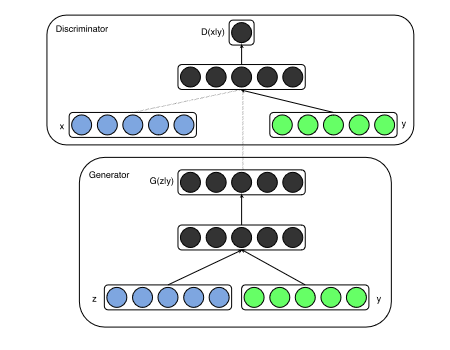
\includegraphics[width=1.2\textwidth]{cgan.png}
	\caption{Conditional Adverserial Network}
	\label{fig:Bild20}
\end{figure}

\subsection{3D-GAN}

Das besondere an den 3D Raum im Vergleich zu Normalen 2D Bildern ist die Steigerung der Dimension und zu gleich der hohe Informationsgehalt welcher in 3D Objekten steckt. Das Ziel von 3D-GAN ist es die Datenverteilung der zugrunde liegenden 3D-Modellen zu erlernen. Dabei wird der latente Objektraum erfasst und soll dadurch die Wahrscheinlichkeiten für einzelne Objektklassen enthalten. 
\\
Es wurden schon mehrere Versuche von generativen Modellen auf 3D Daten durchgeführt wie von Wu, Jiajun und Zhang \cite{3d} welche in ihren Model mit mit 3D-Voxel Daten arbeiten und damit ein GAN trainiert haben oder Achlioptas, Panos und Diamanti\cite{3dgan} welche ein GAN auf Punktwolken trainiert. Da in folgender Arbeit die 3D-Daten durch PC dargestellt werden wird das Vorgehen von Achlioptas, Panos und Diamanti näher beleuchtet.
\\
Die Architektur des typischen 3D-GAN in dieser Arbeit als RAW-GAN betitelt ist dem Vanilla GAN von Goodfellow ähnlich. Der Input Layer ist ein Fully-Connected Layer welcher der Anzahl der Punkte je Punktwolke * 3 entspricht. Dieser bekommt als Input einen Noise-Vektor welcher aus einer Gausischen Verteilung entnommen wird und durch mehrere Layern gereicht bis hin zum Output Layer welche die Anzahl der gewünschten Punkte besteht. Also Zielfunktion kann mit der KL-Zielfunktion gearbeitet werden oder mit der Wasserstein Metrik welche im Versuchsaufbau von Achlioptas, Panos und Diamanti besser Ergebnissee geliefert hat. Der Aufbau unterscheidet sich nicht von Vanilla-GAN. 
\\
Eine weitere Möglichkeit ist das Latent-GAN, dieses benutzt eine andere Aufbau gegenüber dem RAW-GAN, welches dabei helfen soll den latenten Raum der Objekte zu erlernen. Zunächst wird ein Autoencoder mit den vorhanden Trainingsdaten(siehe Autoencoder) trainiert. Der Aufbau ist der selbe einen üblichen Autoencoder beschrieben in Kapitel "Autoencoder". Ziel dabei ist den latenten Raum der Trainingsdaten zu erlernen und eine Kompression der Daten um den Suchraum zu  welcher beim RAW-GAN durch die Inputdimension gegeben ist zu verringern und dadurch das Training des GANs zu erleichtern. 
\\
Bevor das Training des Latent-GAN beginnen kann wird nun meine Trainingsdaten durch den vorher trainierten Encoder des 3D-Autoencoder auf die festgelegte Output-Dimension komprimiert. Anschließend werden diese komprimierten Daten verwendet um das GAN zu trainierten. Dabei erlernt das GAN komprimierte Code zu produzieren welche anschließend durch den Decoder des 3D-Autoencoder wieder auf die ursprüngliche Größe gebracht werden kann. Durch dieses Verfahren war es ihnen Möglich Daten in einer guten Qualität zu produzieren und eine Datenverteilung des zugrundeliegenden Models zu erlernen. Der gesamte Ablauf kann in \ref{fig:Bild30} entnommen werden. 

\begin{figure}[htbp] 
	\centering
	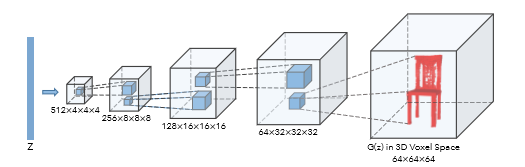
\includegraphics[width=1.2\textwidth]{3dgan.png}
	\caption{Latent-GAN}
	\label{fig:Bild30}
\end{figure}
\cite{3d}

\subsection{Rekonstruktion von Daten}

Derzeit setzt Deep Learning neue Maßstäbe bei der Rekonstruktion von Daten wie Bildern oder Texte. Bei der Rekonstruktion geht es darum das Daten welche von ihren Urzustand verändert wurden, sei es durch Artefakte oder manuelle Bearbeitung wieder dahin zurück zu führen. In Abb. \ref{fig:Bild40} ist eine Rekonstruktion eines Bildes dargestellt welches eine Wiederherstellung eines Hundes zeigt. Deep Learning hat in diesen Bereich besonders bei Bilder große Erfolge erlangt, dadurch das diese als Matrizen dargestellt werden können liefern sie eine Datenstruktur auf welche KNN arbeiten können. Auch durch Bearbeitung mit Convolutionen-Layer auf Bilddaten zählt als Erfolg für die Weiterverarbeitung\cite{imagerecon}. Durch die genannten Methoden werden bessere Strukturen für das jeweilige Ziel, in diesem Fall der Rekonstruktion gelernt und ermöglicht es wie in verschieden Papern wie \cite{imagere1}  welche auf super-hochauflösenten Bildern Artifakte entfernt und das Bild wieder zum Urzustand zurück führt.
Ebenso wie die Arbeit von Liu, Gulin und Reda \cite{imagere2} welche ähnliche Ergebnisse liefern konnte. Rekonstruktion auf 3D-Daten wurde von Yi, Li und Shao \cite{3d_recon} durchgeführt diese Arbeiteten beinhaltet jedoch die Rekonstruktion von 2D Bildern auf 3D Modellen. Bei wurde mit Hilfe von Autoencoder gearbeitet welche auf für die folgenden Arbeit von Bedeutung sind.\cite{3d_recon}. 

\begin{figure}[htbp] 
	\centering
	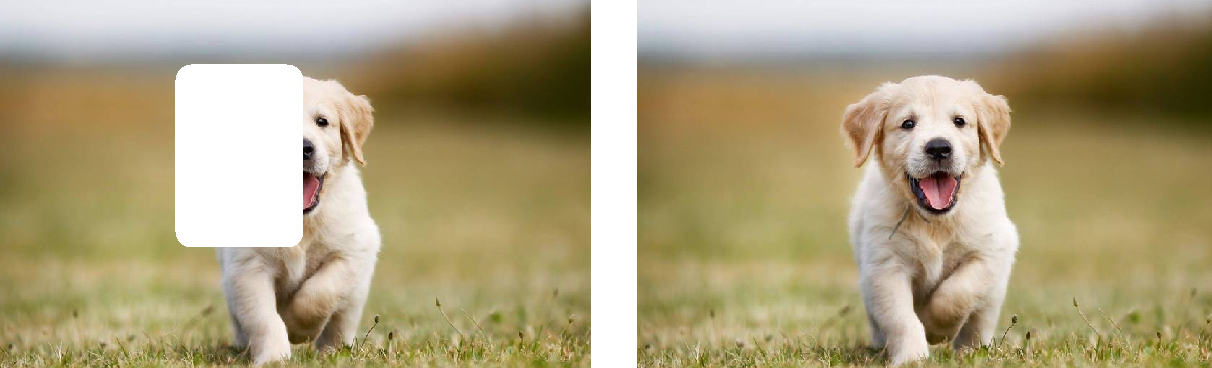
\includegraphics[width=1.2\textwidth]{imagere.png}
	\caption{Bild Rekonstruktion eines Hundes welches durch ein Artefakt zerstört wurde}
	\label{fig:Bild40}
\end{figure}


\section{Methoden}
In diesen Kapitel werden die Methoden für die Versuchsaufbauten aufgezeigt welche die Ziele 1 - 3 überprüfen sollen. Es wird zunächst ein generelle Struktur des Aufbaus besprochen und anschließend auf spezifische gegebeneingeganngen. Außerdem werden die spezifischen Datensätze für die jeweiligen Datensätze aufgezeigt und ihre enstehung erläutert. Alle Versuche wurden auf einen Computer mit Ubuntu 14.05 Betriebssystem mit einen IntelR CoreTM i7-7700k mit 4.50GHz einer Geforce GTX 1089 mit 8G Grafikspeicher. Training und Testen wurden mit CUDA 9.0 und cudNN 7.1.1.

\subsection{Aufbau}
\subsubsection{Datensatz 1. Versuchsaufbau}
Der erste Datensatz "Stühle" besteht aus 4014 Punktwolken mit je 2056 Punkten. Der Datensatz wurde aus von den Shapenet Datensatz entnommen. Ein Beispielpunktwolke kann aus Abbildung entnommen werden. Er ist als .ply Datenformat abgespeichert. 

 Die Daten für den zweiten Datensatz "Blätter" stammen vom Fraunhofer Institut. Der Grunddatensatz bestand aus mehreren 3D-Scans von Tabakpflanzen bei den die Blätter der Pflanze zu einen Datensatz zusammengefügt wurden sind. Der "Blätter" Datensatz besteht aus 420 Punktwolken mit je 2056 Punkten. Er ist als .ply Datenformat abgespeichert.
\begin{figure}[htbp] 
	\centering
	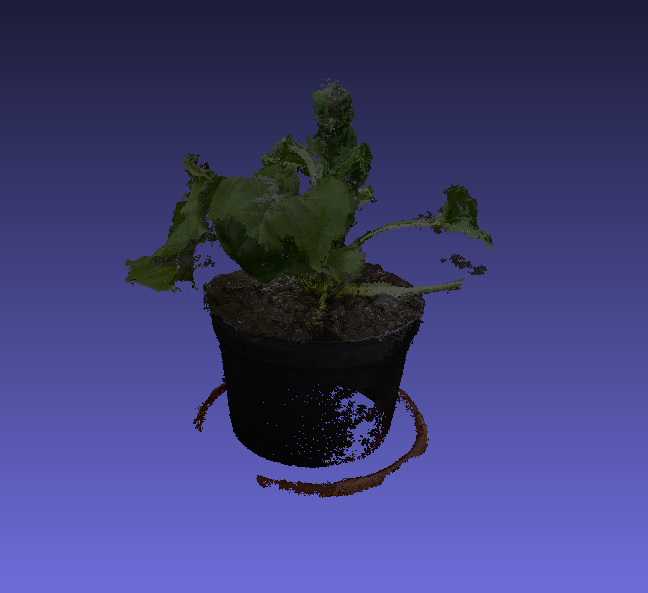
\includegraphics[width=1.2\textwidth]{plant.png}
	\caption{3D Punktwolke einer Tabakpflanze}
	\label{fig:Bild2}
\end{figure}

\begin{figure}[htbp] 
	\centering
	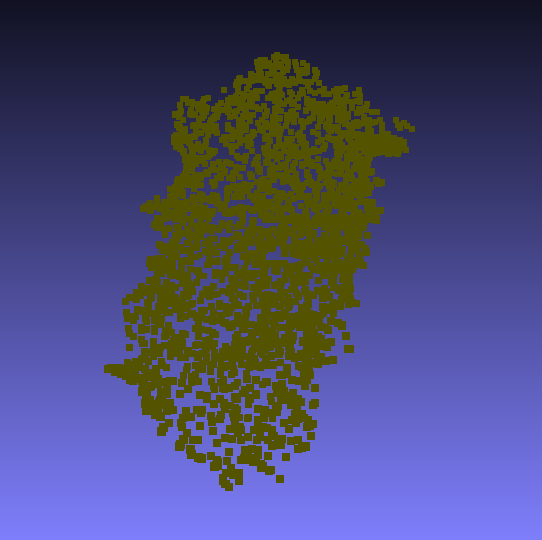
\includegraphics[width=1.2\textwidth]{leaf1.png}
	\caption{3D Punktwolke einer Tabakpflanze}
	\label{fig:Bild2}
\end{figure}

\subsubsection{Datensatz 2. Versuchsaufbau}

Für den zweiten Versuchsaufbau wird auf den in Datensatz Versuchsaufbau 1. Blatt Datensatz "Blätter" zurück gegriffen. Dabei wird in den Blättern punkte heraus genommen welche das verdecken oder zerstört sein eines Blattes simulieren soll. Dies passiert indem eine Gäußverteilung auf einer 3D-Sphere erzeugt wird. Anschließend wird das Komplement zwischen einem 3D-Blatt und einer 3D-Sphere berechnet das Ergebnis sind zerstörte Blätter mit Kreisrunden Löchern auf der Oberfläche. Der Algrorithmus zum erzeugen der Trainingsdaten kann im Anhang entnommen werden. In Abbildung sind die 3 Abschnitte zu erkennen wie die Trainingsdaten erzeugt werden. 
\begin{figure}[htbp] 
	\centering
	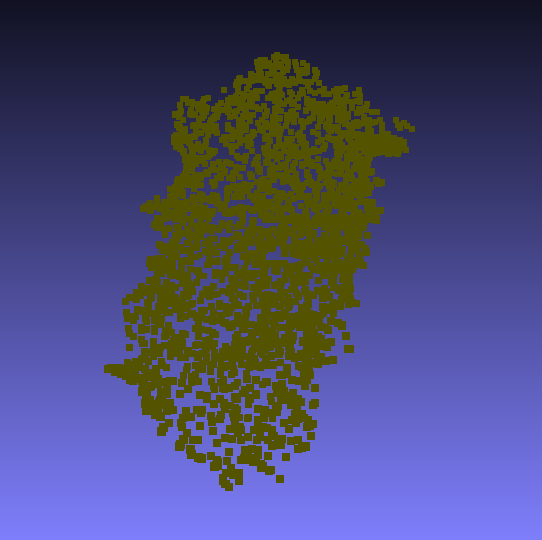
\includegraphics[width=1.2\textwidth]{leaf1.png}
	\caption{3D Punktwolke einer Tabakpflanze}
	\label{fig:Bild2}
\end{figure}

Insgesamt besteht der Trainingsdatensatz aus 450 unzerstörten Blättern sowie 1024 zerstörten paaren. 
\subsubsection{Trainingsaufbau 1 - GAN}
Der Aufbau besteht aus zwei unterschiedlichen Versuchen. Aufbau 1 ist der RAW - GAN Aufbau. Dabei wird auf den herkömmlichen Aufbau von GAN zurückgegriffen. Die Algemeinen Meta-Trainingsvariablen sind Learningrate mit 0,005 und einen AdamOptimizer, mit einem Beta1 von 0.5 und einem Beta2 von 0,5Der Discriminator besteht aus 4-Layern welche 1-Dimensionaler Convolutional Layer bestehen. Mit einer Kernel Größe von 1 und stride von 1. Die Aktivierungsfunktion sind Relus. Darauf folgt 3 fully connected Layer mit der Größe 128, 54 und 1 alle mit einer Relu Aktivierungsfunktion.
\\
Der Generator besteht auf 5 fully-connected Layern mit [64,128,512,1024,1536] neuronen jeweils mit einer Relu Aktivationsfunktion. Der Aufbau kann in Abbildung entnommen werden. Die Zielfunktion ist die Wasserstein Metric und die übliche GAN Zielfunktion. 

Der Versuchsaufbau 2ist das Latent-GAN zunächst wird dabei der Autoencoder mit den Trainingsdaten trainiert. Der Encoder des Autoencoders wird mit einer Learning Rate von 0.0005 trainiert. und einer Batch Größe von 50. Der Encoder besteht dabei besteht dabei aus 4 1-D Convolutional Layern mit 64,128,246,1024] Filtern Stride von 1 und Size von 1. Die Activierungsfunktion ist relu. Der Letzte Layer ist ein Max Layer. Der Decoder besteht aus aus [256,256,[614]


\subsubsection{Trainingsaufbau 2 - CGAN für Punktwolkenrekunstroktion }

Da sich im Trainingsaufbau 1 das L-GAN bessere Ergebnisse liefert bei erlernen von Punktwolken Daten. Wird der Aufbau von L-GAN übernommen und dahin gehen verändert, das Ziel zu erfüllen. Zunächst werden wie bei Trainingsaufbau 1 die Trainingsdaten(siehe Trainingsdaten Aufbau 2) trainiert. Der Aufbau des Autoencoder ist dabei gleich dem von Aufbau 1. Der Encoder des Autoencoders wird mit einer Learning Rate von 0.0005 trainiert. und einer Batch Größe von 50. Der Encoder besteht dabei besteht dabei aus 4 1-D Convolutional Layern mit 64,128,246,1024] Filtern Stride von 1 und Size von 1. Die Activierungsfunktion ist relu. Der Letzte Layer ist ein Max Layer. Der Decoder besteht aus aus [256,256,[614]. Die Zielfunktion ist die Champfer Disdance  da sie die besten Ergebnisse bei citiere PGAN besten geliefert hat.\\

Anschließend werden zerstörten BlatDaten x mit den trainierten Encoder zu den latenten Code y komprimiert, der einen Vektor von 128-D entspricht.
Das selbe wird mit den unzerstörten Blattdaten x`gemacht welche mit den Encoder zu dem latenten Code y`komprimiert werden welcher einen Vektor von 128-D entspricht. Wobei es jeweils (x,x`) paare Gibt welche den 

Der Aufbau des C-GANS entspricht der in im 3.4 beschrieben C-GAN üblichen Aufbau. der Generator bekommt als Input x' und x welches einen 128-D Vektor welcher aus einer Gausischen Verteilung gesamplet wird. Der Generator besteht aus 3 layern [256,128,128] der Diskriminator besteht aus 2 fully Connectected Layer mit der Größe [128,128]\\ Bei generator und Diskriminator wird beim Trainieren jeweils Batchnormalization eingesetzt. 

Als Zielfunktion wird wieder das W-GAN verwendet da es im Versuchsaufbau 1 die besseren Ergebnisse liefert. \section{Evaluation und Ergebnise}
Es wird nun in diesen Kapitel auf die Ergebnisse von Versuchsaufbau 1 und 2 eingeganngen. Zunächst wird Versuchsaufbau 1 mit des erlernen von latenten Raum von Punktwolken gezeigt. Anschließend geht es um die Ergebnisse von Versuchsaufbau 2 für die Rekunstruntion von zerstörten Blättern. 

\subsection{Ergebnisse - Versuchsaufbau 1}

Die Ergebnisse von RAW-GAN mit den Blattdaten welches nach 500 Epochen Training lassen sich in Abb. entnehmen. Wie zu sehen ist sind die Blätter nicht gut genug für eine Weiterverarbeitung. Die Daten erinnern eher an einen hohlen Ball als an Blättern. Auch lässt der Trainingsverlauf aus Abb. zu entnehmen darauf schließen das keine weitere Verbesserung möglich ist auch auf längere Epochen gesehen da es zu viele Sprünge in der Zielfunktion den Discriminator zu gut werden lässt und den Generator nicht verbessern lässt. 

\begin{figure}[htbp] 
	\centering
	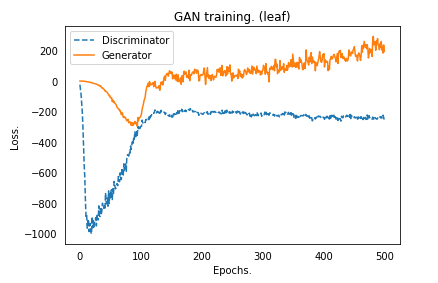
\includegraphics[width=1.2\textwidth]{raw_gan_leaf_result.png}
	\caption{Trainingsverlauf des RAW-GAN mit den Blattdaten}
	\label{fig:Bild35}
\end{figure}
\begin{figure}[htbp] 
	\centering
	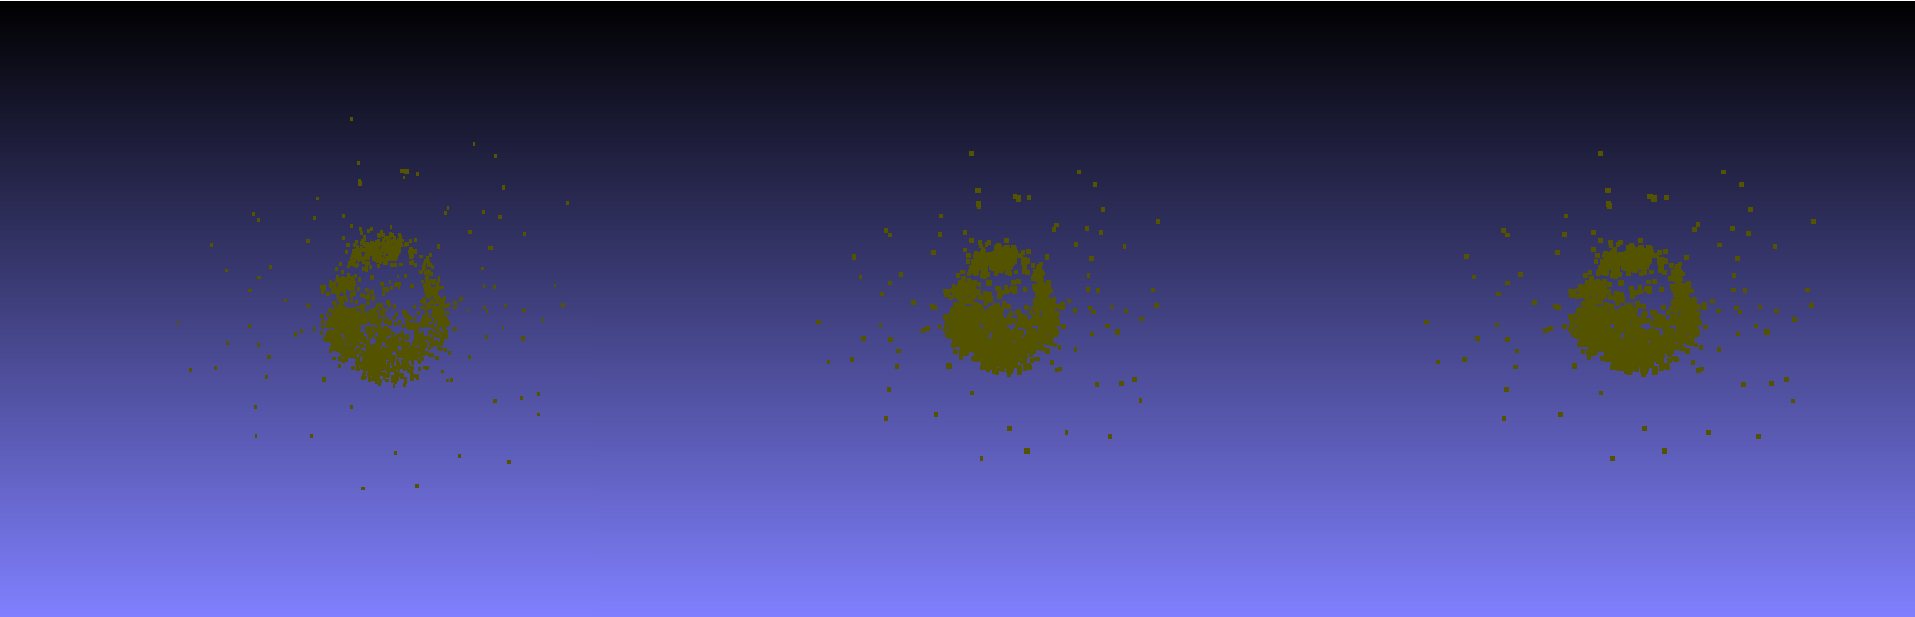
\includegraphics[width=1.2\textwidth]{raw_gan_leaf_example.png}
	\caption{Traingsverlauf des RAW-GAN mit den Blattdaten}
	\label{fig:Bild36}
\end{figure}

Ähnliche Ergebnisse sind auch mit den Stuhldaten zu beobachten in Abb. jeweils die Ergebnisse dafür. Es sind besser die Strukturen zu erkennen als bei den Blättern ebenfalls nicht obtimale Ergebnisse. In Abb. der Trainingsverlauf. 
\\\\

\begin{figure}[htbp] 
	\centering
	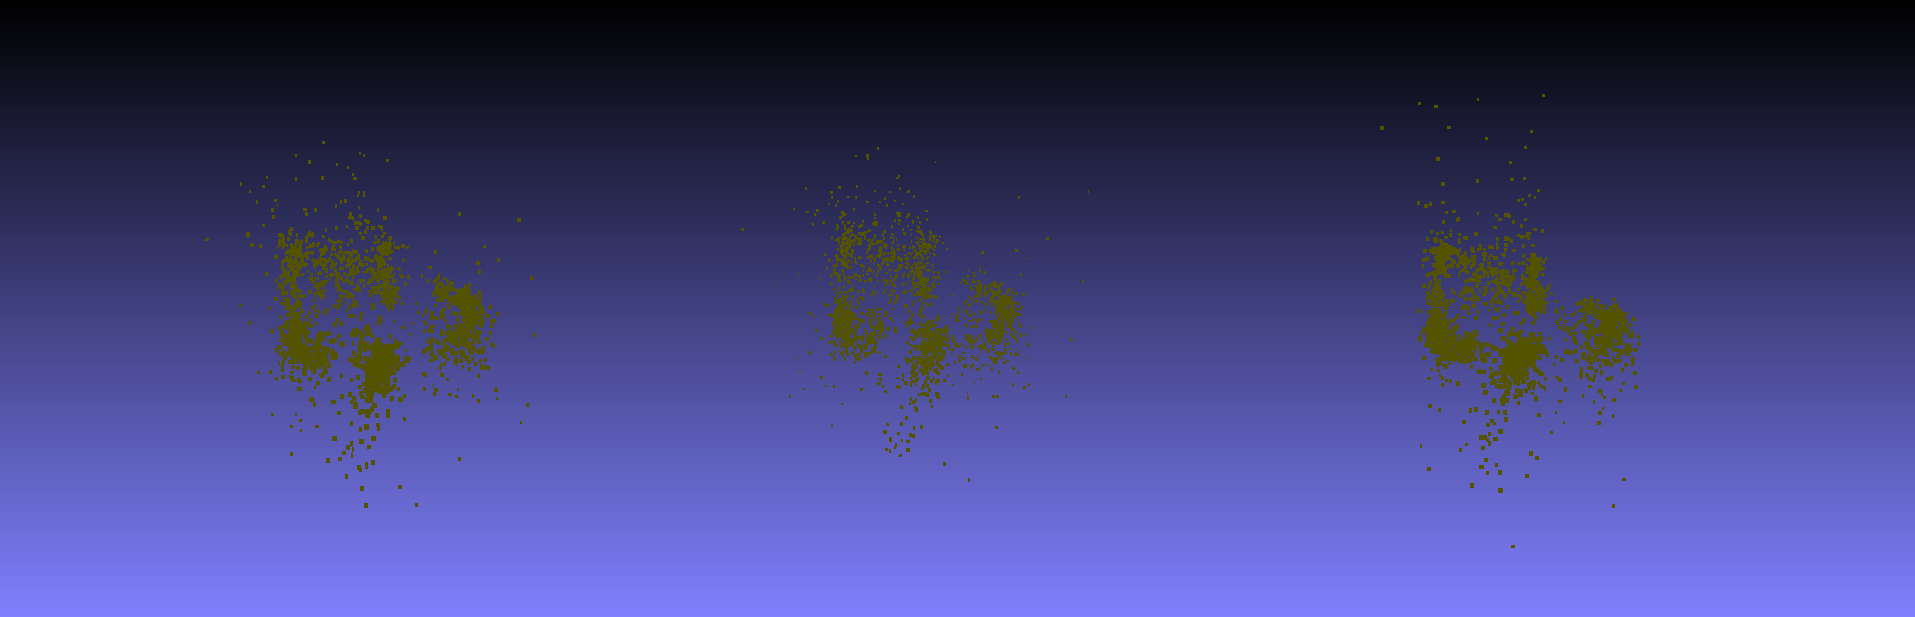
\includegraphics[width=1.2\textwidth]{raw_gan_result_400_result.png}
	\caption{Traingsverlauf des RAW-GAN mit den Stuhldaten mit 422 Trainingsdaten}
	\label{fig:Bild35}
\end{figure}
\begin{figure}[htbp] 
	\centering
	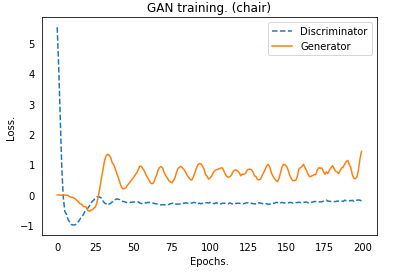
\includegraphics[width=1.2\textwidth]{raw_gan_result_400_examples.png}
	\caption{Traingsverlauf des RAW-GAN mit den Stuhldaten mit 422 Trainingsdaten}
	\label{fig:Bild36}
\end{figure}

\begin{figure}[htbp] 
	\centering
	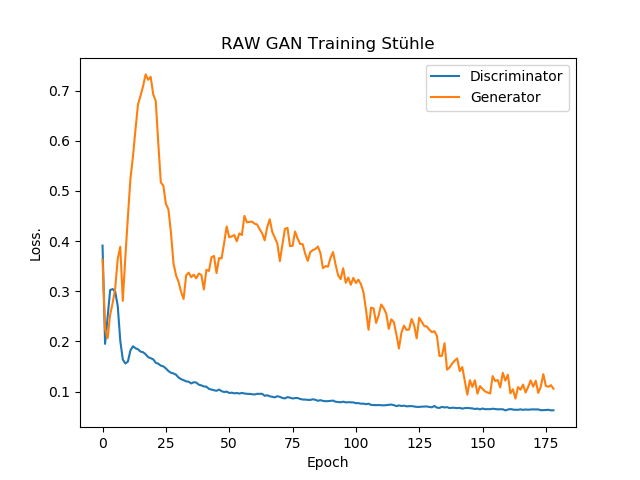
\includegraphics[width=1.2\textwidth]{raw_gan_chair_result.png}
	\caption{Traingsverlauf des RAW-GAN mit den Stuhldaten}
	\label{fig:Bild37}
\end{figure}
\begin{figure}[htbp] 
	\centering
	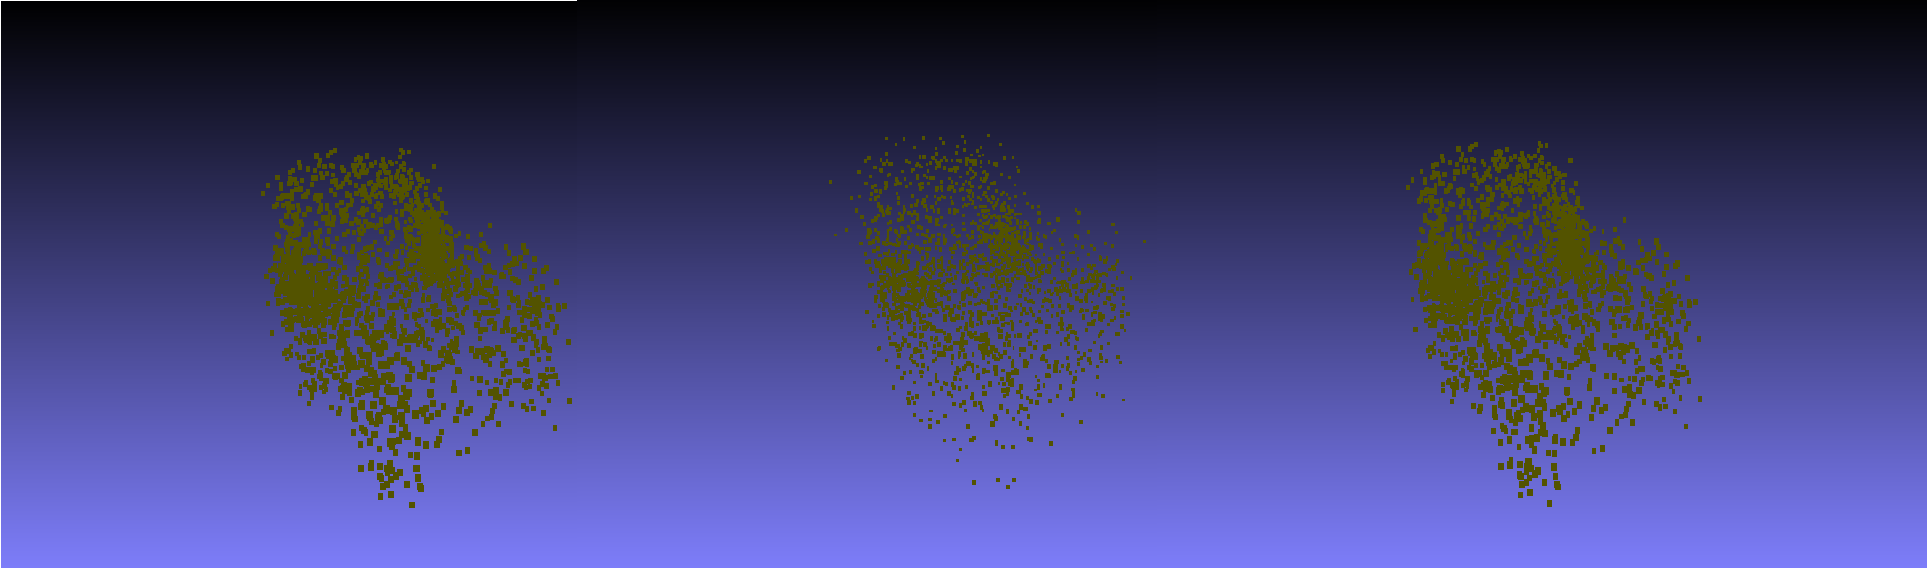
\includegraphics[width=1.2\textwidth]{raw_gan_chair_example.png}
	\caption{Traingsverlauf des RAW-GAN mit den Stuhldaten}
	\label{fig:Bild38}
\end{figure}
Latent-GAN chair
\begin{figure}[htbp] 
	\centering
	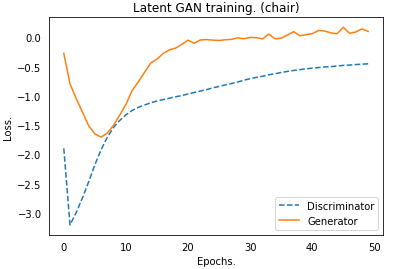
\includegraphics[width=1.2\textwidth]{latent_gan_chair_result.png}
	\caption{Traingsverlauf des Latent-GAN mit den Stuhldaten}
	\label{fig:Bild37}
\end{figure}
\begin{figure}[htbp] 
	\centering
	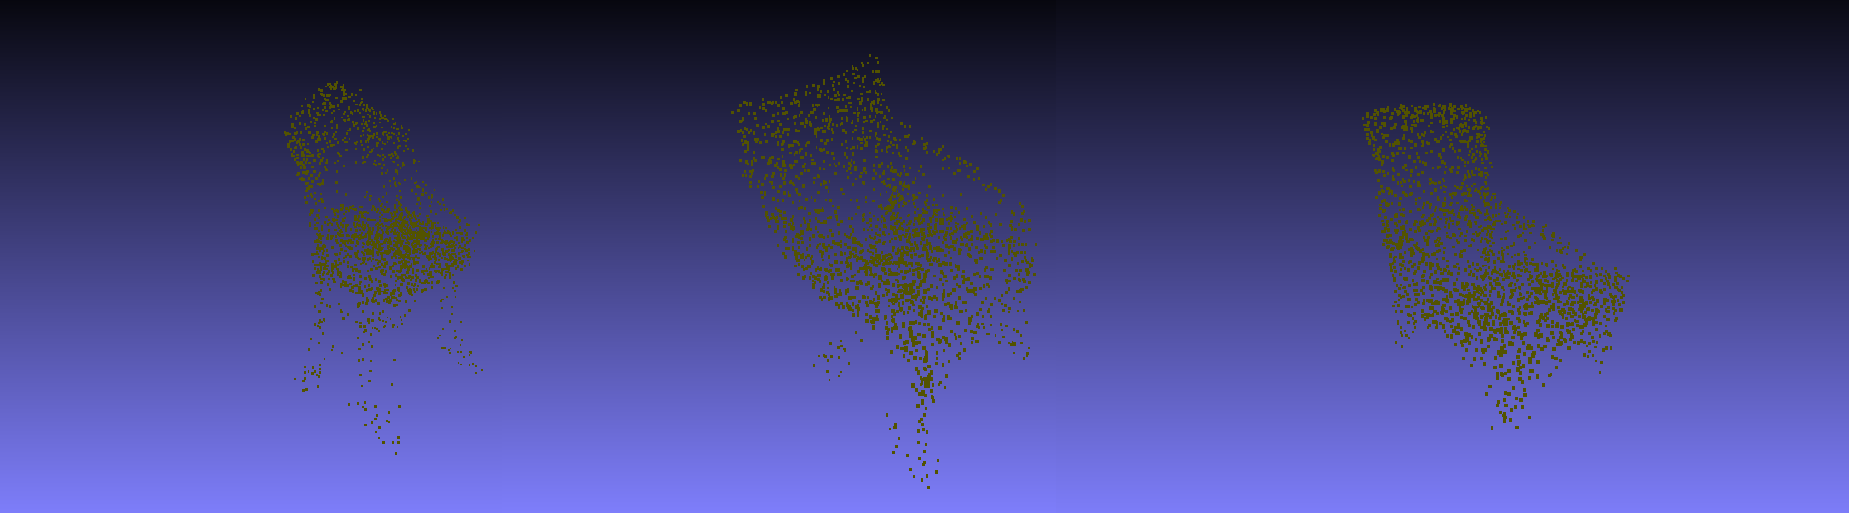
\includegraphics[width=1.2\textwidth]{latent_gan_chair_example.png}
	\caption{Traingsverlauf des Latent-GAN mit den Stuhldaten}
	\label{fig:Bild38}
\end{figure}
Latent-GAN leaf
\begin{figure}[htbp] 
	\centering
	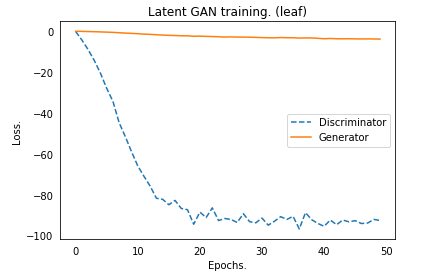
\includegraphics[width=1.2\textwidth]{Latent_gan_training_result.png}
	\caption{Trainingsverlauf des Latent-GAN mit den Blattdaten}
	\label{fig:Bild37}
\end{figure}
\begin{figure}[htbp] 
	\centering
	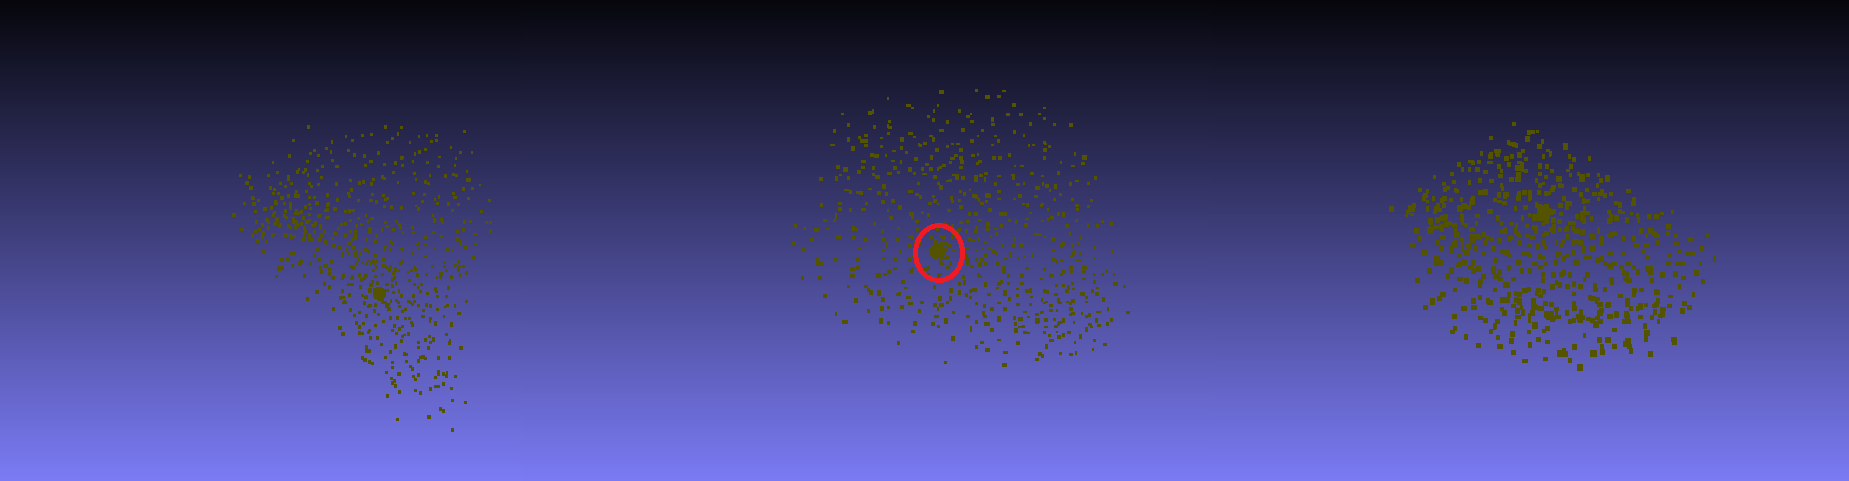
\includegraphics[width=1.2\textwidth]{latent_gan_leaf_example.png}
	\caption{Trainingsverlauf des Latent-GAN mit den Blattdaten}
	\label{fig:Bild38}
\end{figure}
\begin{figure}[htbp] 
	\centering
	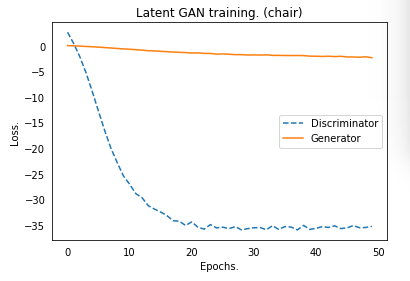
\includegraphics[width=1.2\textwidth]{raw_gan_latent_gan_chair_result_400_example.png}
	\caption{Trainingsverlauf des Latent-GAN mit den Stuhldaten und 400 Trainingsdaten}
	\label{fig:Bild37}
\end{figure}

\begin{figure}[htbp] 
	\centering
	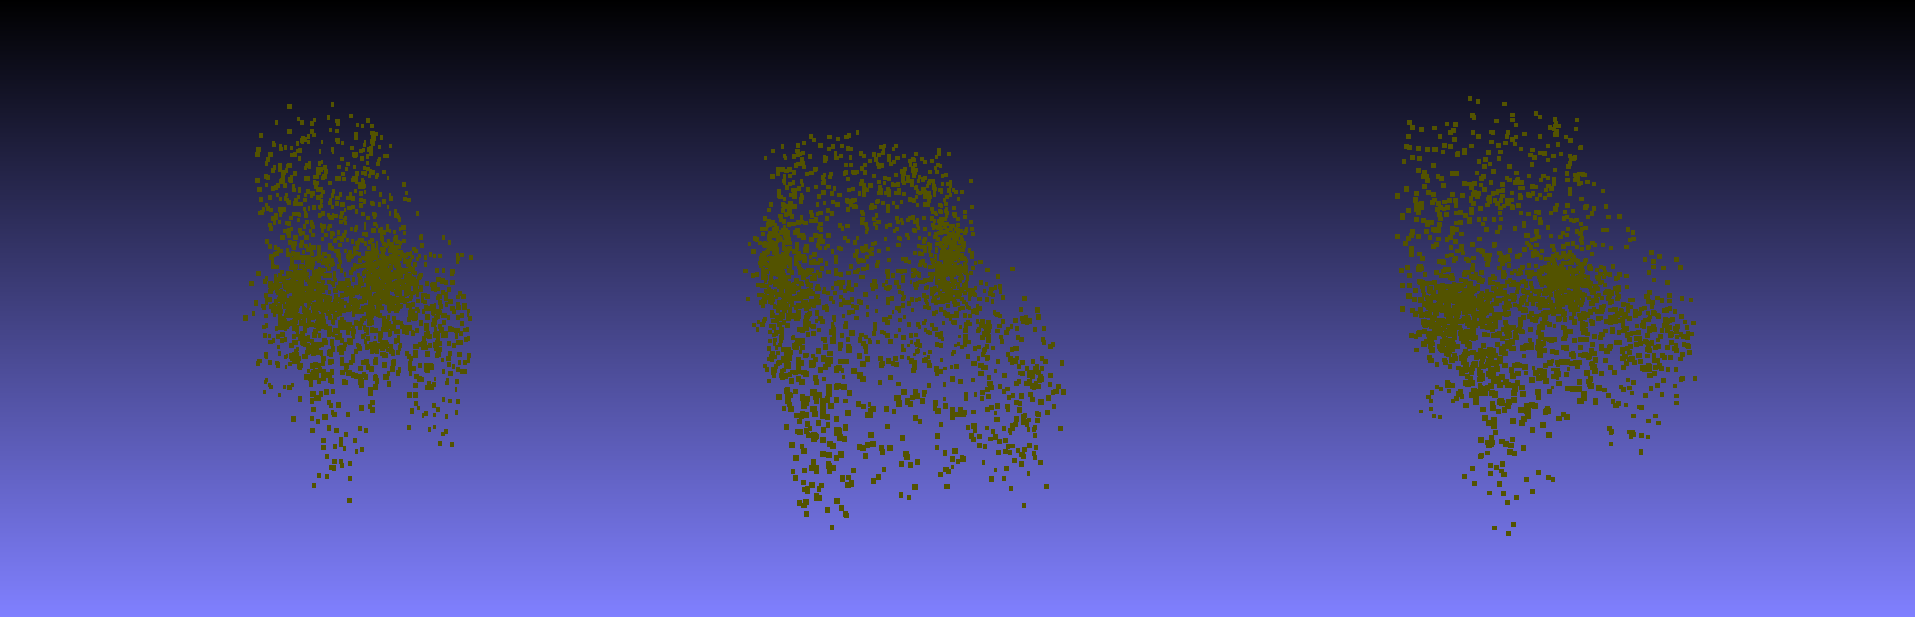
\includegraphics[width=1.2\textwidth]{raw_gan_latent_gan_chair_example_400.png}
	\caption{Trainingsverlauf des Latent-GAN mit den Stuhldaten und 400 Trainingsdaten}
	\label{fig:Bild37}
\end{figure}
\subsection{Ergebnisse - Versuchsaufbau 2}

Die Ergebnisse für das Latent-GAN mit den Blattdaten welches zunächst für 500 Epochs mit den Autoencoder trainiert wurde können Input und Output Paare aus Abbildung entnommen werden in Abbildung sind die Loss jeweils mit EMD-Loss und Damfer Distanz aufgelistet.
\\\\
Die Ergebnisse für das Latent-GAN mit den Tischdaten welches zunächst für 500 Epochs mit den Autoencoder trainiert wurde können Input und Output Paare aus Abbildung entnommen werden in Abbildung sind die Loss jeweils mit EMD-Loss und Damfer Distanz aufgelistet.
\begin{figure}[htbp] 
	\centering
	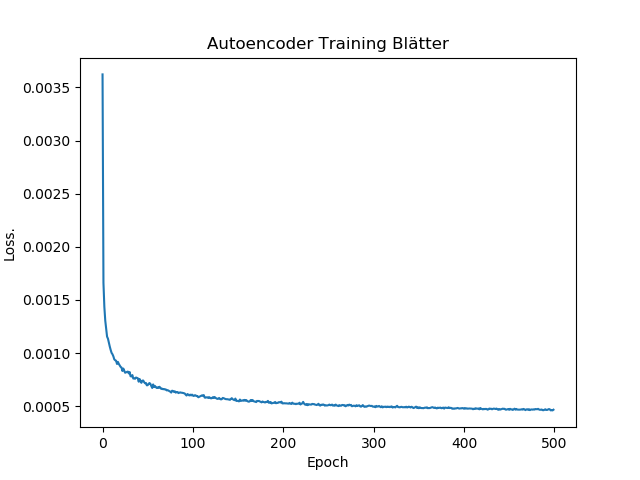
\includegraphics[width=1.2\textwidth]{autoencoder_training_blaetter_result.png}
	\caption{Trainingsverlauf des RAW-GAN mit den Blattdaten}
	\label{fig:Bild42}
\end{figure}

\begin{figure}[htbp] 
	\centering
	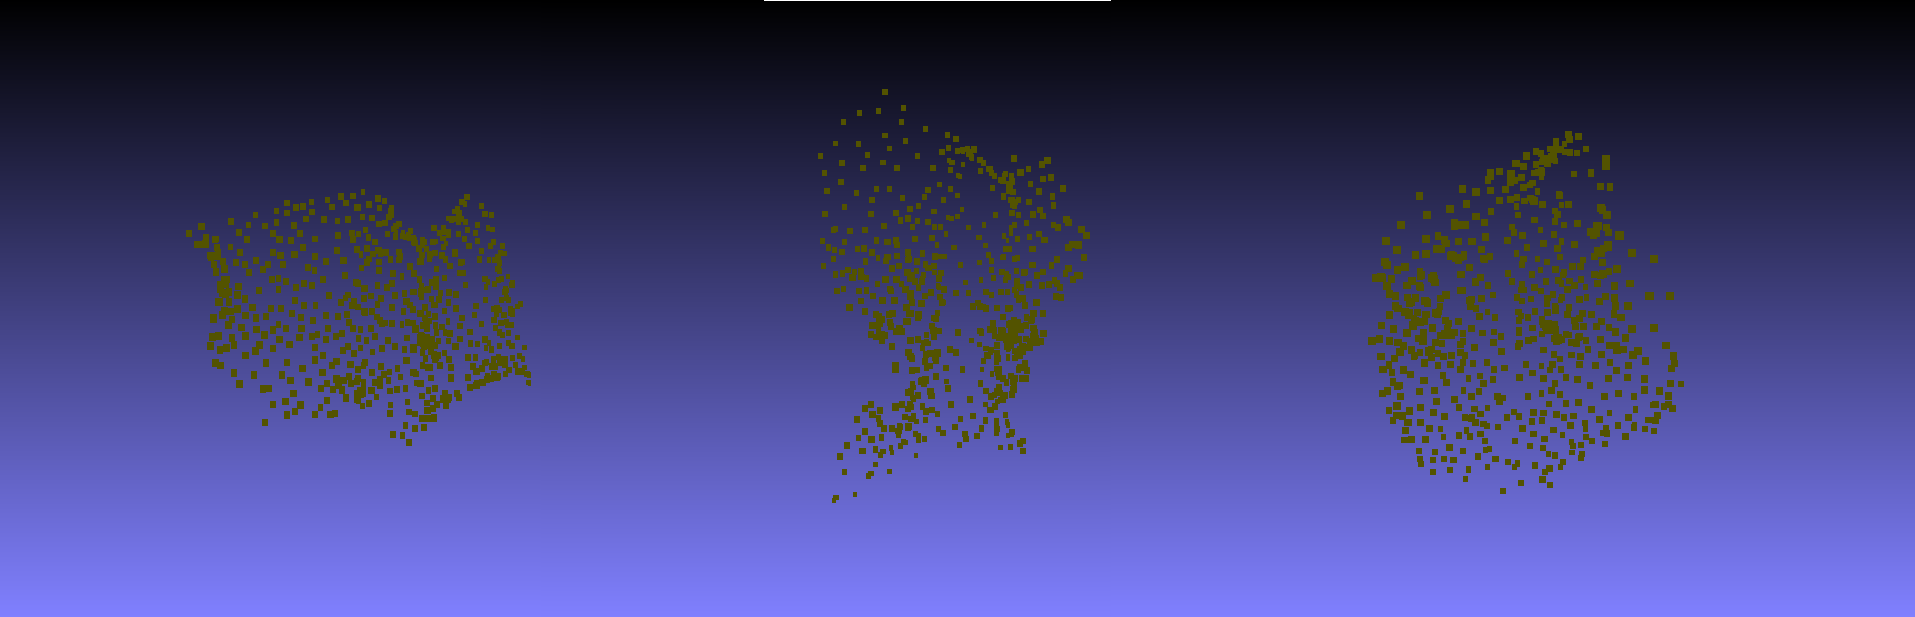
\includegraphics[width=1.2\textwidth]{autoencoder_destroyed_example_chamfer_fake.png}
	\caption{Trainingsverlauf des Autoencoders mit den zerstörten Blattdaten CD Output}
	\label{fig:Bild43}
\end{figure}

\begin{figure}[htbp] 
	\centering
	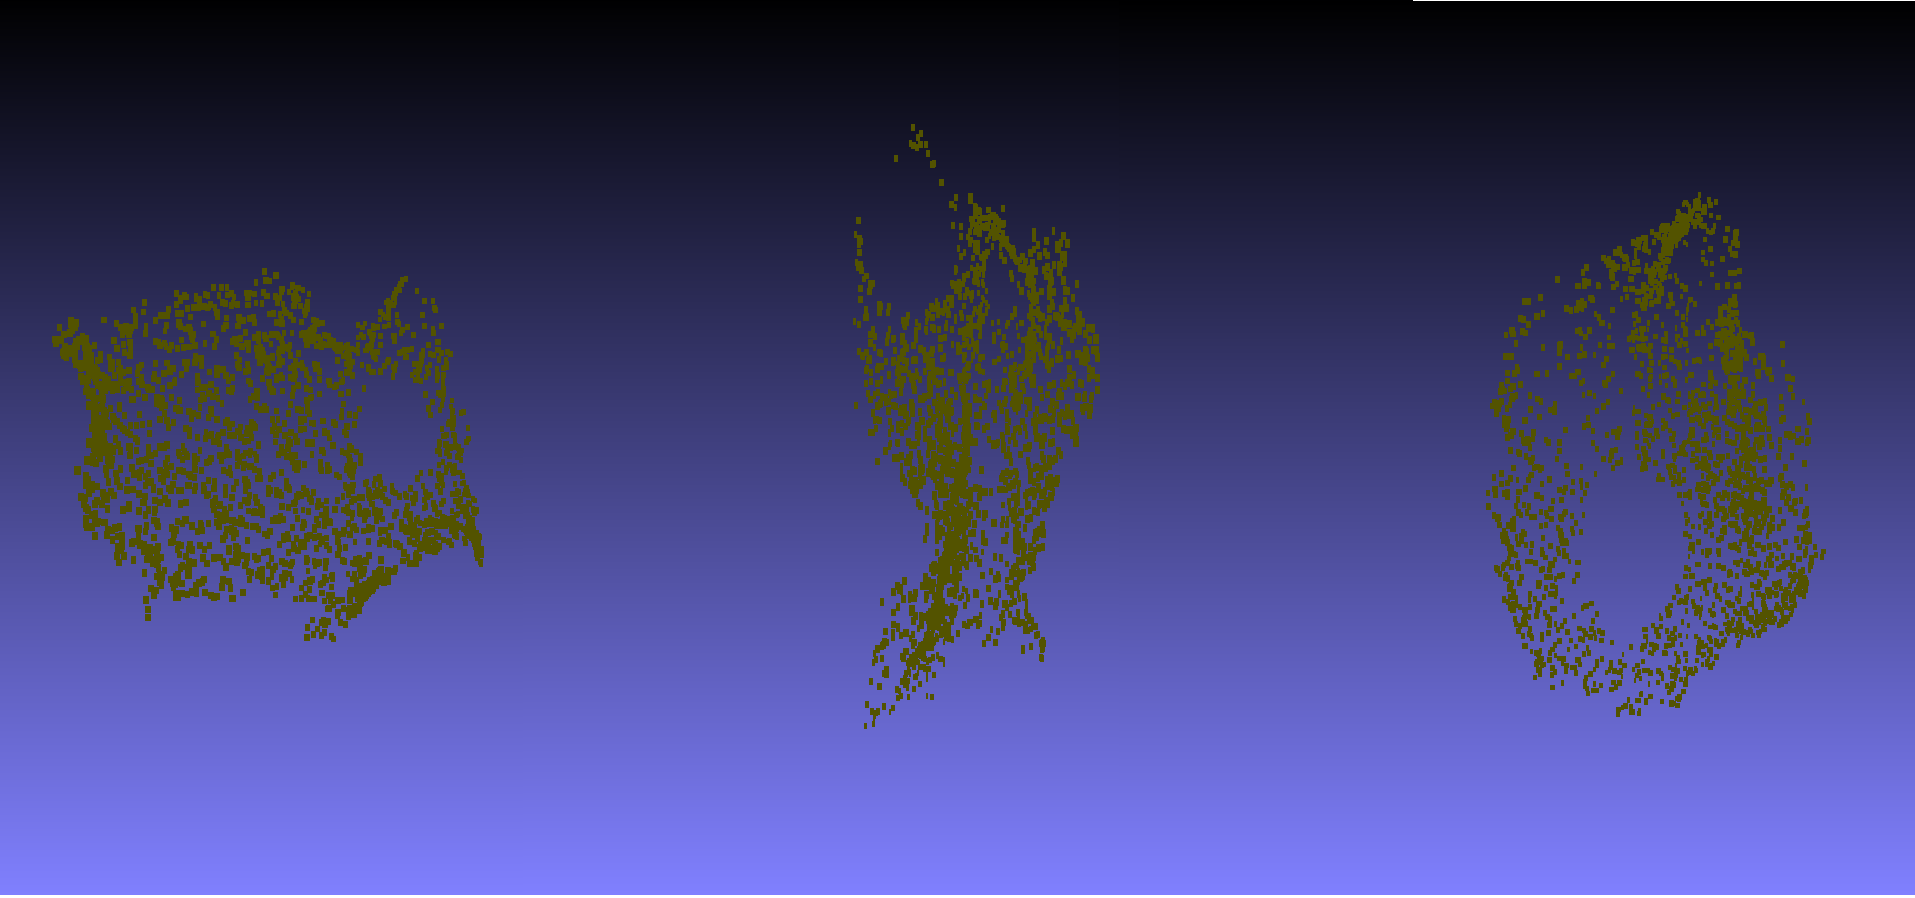
\includegraphics[width=1.2\textwidth]{autoencoder_destroyed_example_chamfer_real.png}
	\caption{Trainingsverlauf des Autoencoders mit den zerstörten Blattdaten CD input }
	\label{fig:Bild43}
\end{figure}

\begin{figure}[htbp] 
	\centering
	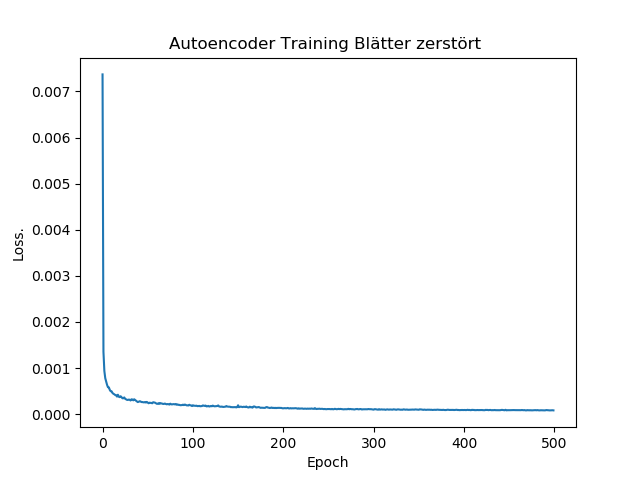
\includegraphics[width=1.2\textwidth]{autoencoder_training_bleatter_zer_result.png}
	\caption{Trainingsverlauf des Autoencoders mit den zerstörten Blattdaten CD}
	\label{fig:Bild43}
\end{figure}

\begin{figure}[htbp] 
	\centering
	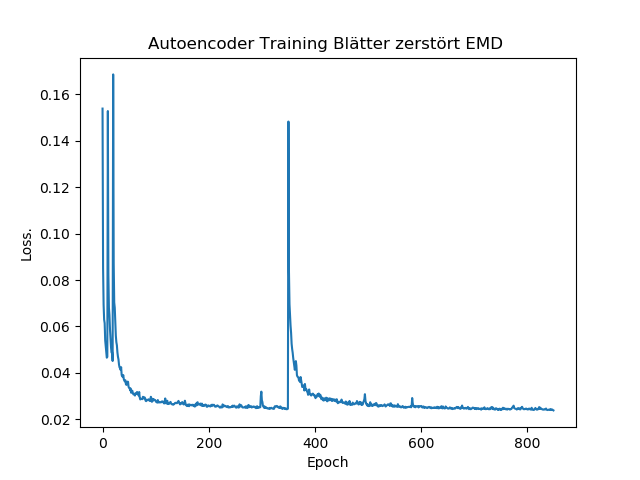
\includegraphics[width=1.2\textwidth]{autoencoder_training_bleatter_zer_result_emd.png}
	\caption{Trainingsverlauf des Autoencoders mit den zerstörten Blattdaten EMD}
	\label{fig:Bild44}
\end{figure}
\begin{figure}[htbp] 
	\centering
	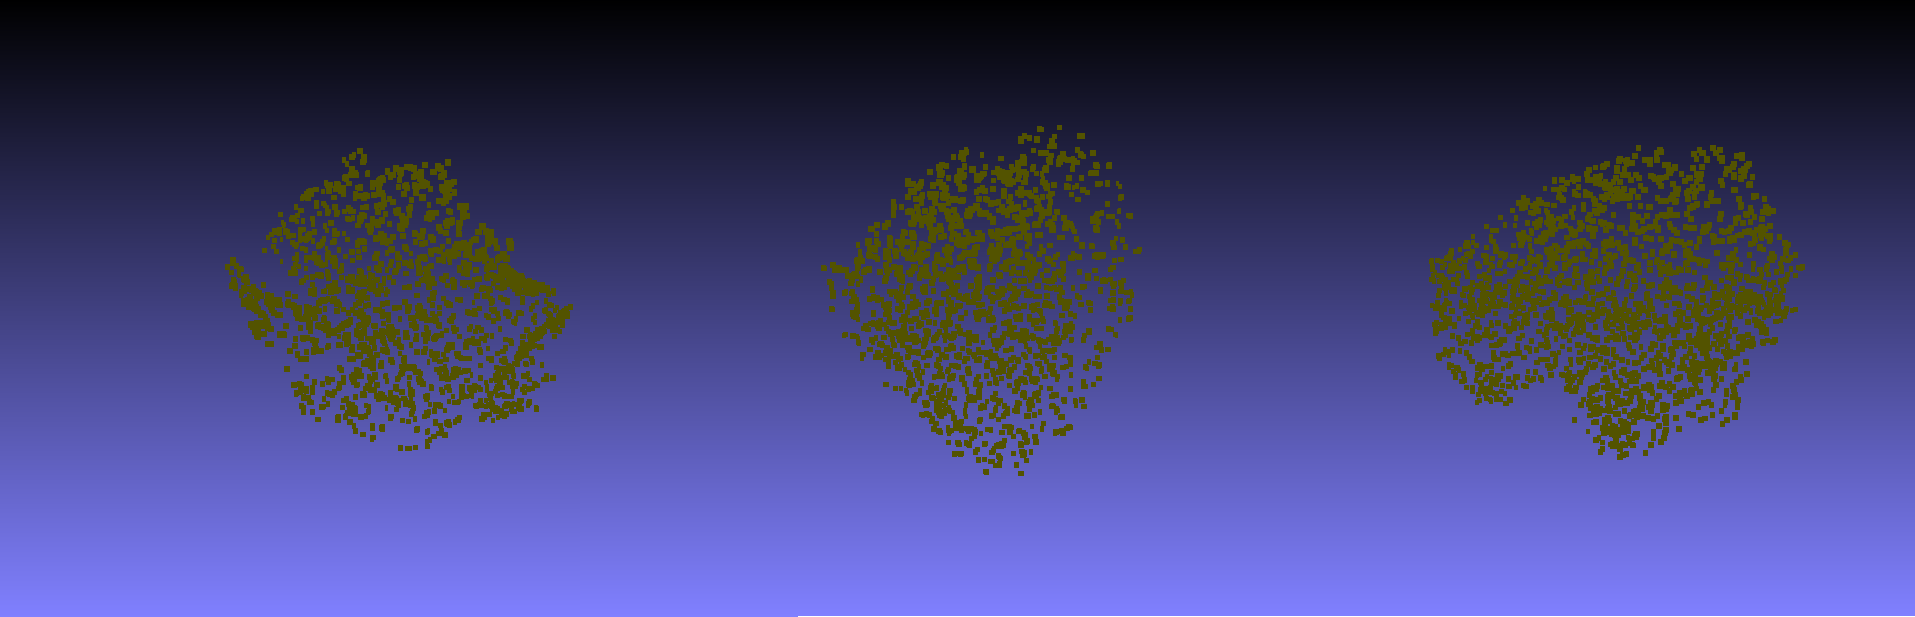
\includegraphics[width=1.2\textwidth]{autoencoder_destroyed_example.png}
	\caption{Trainingsbeispiele des Autoencoders mit den zerstörten Blattdaten EMD}
	\label{fig:Bild44}
\end{figure}



\section{Zusammenfassung und Diskussion }
Ein GAN besteht aus zwei ANN, dem Discriminator und dem Generator. Das Ziel des G ist es Daten zu erzeugen, welche nicht von Trainingsdaten unterschieden werden können. Der Discriminator hat die Aufgabe zu unterscheiden ob der jeweilige Datensatz von G erzeugt wurde und somit ein fake Datensatz ist, oder von den Trainingsdaten stammt\cite{goodfellow2014}. GANs werden derzeit noch erforscht. Es gibt noch einige offene Fragen, beispielsweise bezüglich der Performance hochauflösender Bilder\cite{ende}. Es wurden in diesem Paper einige Probleme, welche beim Trainieren von GAN auftreten können und mögliche Lösungsansätze, vorgestellt. Es gibt derzeit einige praktische Ansätze, welche in der Anwendung auf GANs zurück greifen. Beispielsweise durch Textbeschreibung eigene Bilder als Output generiert werden \cite{texttoimage}, oder 3D Daten erzeugt werden\cite{3dgan}. GANs finden Anwendung in unterschiedlichen Bereichen des Deep Learnings, da sie als Lösung des Problems angesehen werden, dass Neuronale Netzwerke eine hohe Menge an Trainingsdaten benötigen und GANs dieses Problem durch ihre Fähigkeit, neue Daten zu generieren, umgehen. GANs lernen eine Art "verstecke" Repräsentation von Klassen, was dazu beitragen kann auch Modelle von komplexen Prozessen zu erlernen. Es gibt erste Ansätze bei denen im Reinforcement Learning durch GANs versucht wird Modelle von der Umwelt eines Agenten zu erlernen, welche dann auf Grundlage dieser Modelle Vorhersagen über zukünftige Ereignisse treffen kann\cite{reinforcment}.
\newpage
\listoffigures
\newpage
\listoftables
\newpage
\bibliographystyle{apacite}
\bibliography{mybib.bib}

\end{document}
